% !TeX spellcheck = en_US
%\documentclass[preprint,authoryear]{elsarticle}
\documentclass[preprint]{elsarticle}
% sudo apt-get install -y texlive-publishers

\usepackage[left]{lineno}
\usepackage[latin1]{inputenc}
\usepackage[T1]{fontenc}
\usepackage{lmodern}
\usepackage{multirow}

\usepackage{lineno,hyperref}
\modulolinenumbers[5]

\usepackage[none]{hyphenat}

\usepackage{url}
\usepackage{booktabs}

\usepackage{tikz}
\usetikzlibrary{calc}
\usetikzlibrary{positioning}

\usepackage{mathtools}
\usepackage{amssymb}
\usepackage{amsthm}

\usepackage{caption}
\captionsetup{labelfont=bf}
\captionsetup{skip=0pt}

\usepackage{pgfplots}
\pgfplotsset{compat=newest}
\usepackage{algorithm}

\usepackage[noend]{algpseudocode}

\usepackage[margin=0.9in]{geometry}

\usepackage[normalem]{ulem}
%\usepackage{xcolor}

\newcommand{\Comentar}[1]{\State {\cmmt{#1}}}
\newcommand{\Break}{\State \textbf{break}}
\renewcommand{\Return}{\State \textbf{return}~}
\renewcommand{\algorithmicensure}{\textbf{Parameters:}}

\renewcommand\algorithmicthen{}
\renewcommand\algorithmicdo{}


\algblock{ForEach}{EndFor}
\algblock{ForDownTo}{EndFor}
\algblock{ForTo}{EndFor}

\newcommand{\Block}[1]{\State #1 \{}
\newcommand{\EndBlock}{\State \}}

\usepackage{scrextend}
\newcommand{\boldm}[1] {\mathversion{bold}#1\mathversion{normal}}
\newcommand{\round}[1]{\ensuremath{\lfloor#1\rceil}}
\usepackage{setspace}
\usepackage{array}
\usepackage{color, colortbl}
\definecolor{Gray}{gray}{0.9}
\hyphenation{cost-ef-fec-tive-ness}

\newcommand{\specialcell}[2][c]{%
	\begin{tabular}[#1]{@{}c@{}}#2\end{tabular}}


\journal{Computers \& Operations Research}


\begin{document}


\begin{frontmatter}

\title{Air cargo load and route planning in pickup and delivery operations}

\author{A.C.P.~Mesquita}
\ead{celio@ita.br}

\author{C.A.A.~Sanches\corref{cor1}}
\ead{alonso@ita.br}
\cortext[cor1]{Corresponding author.}

\address {Instituto Tecnol\'{o}gico de Aeron\'{a}utica - DCTA/ITA/IEC\\
Pra\c{c}a Mal. Eduardo Gomes, 50\\
S\~{a}o Jos\'{e} dos Campos - SP - 12.228-900 - Brazil}


\begin{abstract}

In aerial pickup and delivery of goods in a distribution network, transport aviation faces risks of cargo unbalancing due to the urgency required for loading, for fast take-off, and mission accomplishment, especially in times of crisis, public calamity, short deadlines for contracting customers, or any external pressure for immediate take-off. In addition, there is no technological assistance to help the load and trip planners with the huge number of demands for transport in each hub. This enables other risks, such as improper delivery, excessive fuel burn, and longer than necessary turn-around time. We defined and solved the problem of planning the loading and routing of an aircraft according to a utility score, weight and balance principles, and fuel consumption in a tour of simultaneous pickup and delivery at intermediate hubs. This NP-hard problem, named {\it Air Cargo Load Planning with Routing, Pickup, and Delivery Problem (ACLP+RPDP)}, is mathematically modeled using standardized pallets in fixed positions, obeying center of gravity constraints, delivering each item to its destination, and minimizing fuel consumption costs. We performed multiple experiments with a commercial solver and well-known meta-heuristics on data based on the transport history of the {\it Brazilian Air Force}, and also designed a new method that quickly finds good solutions for a wide range of problem sizes, which solved all test scenarios within an acceptable operational runtime.


\end{abstract}

\begin{keyword}
Load Planning \sep Air Palletization \sep Weight and Balance \sep Pickup and Delivery \sep Vehicle Routing
\end{keyword}

\end{frontmatter}

\label{sec1}
\section{Introduction}


Air cargo transport involves several sub-problems that are difficult to solve. Recently, Brandt and Nickel \cite[p. 401]{BrandtStefan2019} defined the {\it Air Cargo Load Planning Problem} (ACLPP) as four sub-problems: {\it Aircraft Configuration Problem} (ACP), {\it Build-up Scheduling Problem} (BSP), {\it Air Cargo Palletization Problem} (APP) and {\it Weight and Balance Problem} (WBP). Several aspects were considered in this modeling: characteristics of the items to be transported (dimensions, scores, dangerousness, etc.); types and quantities of {\it unit load devices} (ULDs), commonly called pallets; when these pallets are assembled; how items are allocated to pallets; in which positions these pallets are to be placed; how the total cargo weight is balanced; etc. They also presented a comprehensive bibliographic survey of solving methods that had been developed in different situations.

However, there are still other important challenges in air cargo transport that go beyond the definition of the ACLPP, especially with regard to the flight itinerary and the loading and unloading at each destination (or node) of this travel plan. In this context, at least two more important sub-problems can be considered: pickup and delivery operations at each node, called {\it Pickup and Delivery Problem} (PDP), and the search for the lowest cost route, which is the well-known {\it Traveling Salesman Problem} (TSP).

Considering air cargo transport, Table \ref{tab:sa} lists the main works in the literature in chronological order, and the corresponding sub-problems addressed. We also indicate whether the dimensions of the items were taken into account ({\bf 3D} or {\bf 2D}) and which solution method was used: heuristics ({\bf Heu}), integers ({\bf Int}), or linear programming ({\bf Lin}).

\begin{table}[H]
	\centering
	\caption{Air cargo transport: literature, problems and features}  \label{tab:sa}
	\scriptsize
	\renewcommand{\arraystretch}{1.1} 
	\begin{tabular}{r|cc|cc|cc|ccc}
		\toprule
		 Work & {\bf APP}  & {\bf WBP}  &  {\bf PDP}   &{\bf TSP}   & {\bf 2D}  & {\bf 3D}  & {\bf Heu}  & {\bf Int}  & {\bf Lin} \\
		\midrule
		Larsen and Mikkelsen \cite{LarsenMikkelsen1979}  & $.$        & $\bigstar$ & $.$          & $.$        & $.$       & $.$       & $\bigstar$ & $.$        &  $.$ \\
		Brosh \cite{Brosh1981}  & $.$ & $\bigstar$  & $.$   & $.$ & $.$ & $.$   & $.$  & $.$  &  $\bigstar$ \\
		Ng \cite{Kevin1992}  & $.$ & $\bigstar$  & $.$ & $.$ & $.$ &$.$   & $.$  & $\bigstar$  &  $.$ \\
		Heidelberg {\it et al.} \cite{Heidelberg1998}  & $.$ & $\bigstar$  & $.$ & $.$ & $\bigstar$ &$.$   & $\bigstar$  & $.$  &  $.$ \\
		Mongeau and Bes \cite{MongeauBes2003}    & $\bigstar$ & $\bigstar$   & $.$ & $.$ & $.$ & $.$   & $.$  & $\bigstar$  &  $.$ \\
		Fok and Chun \cite{fok2004optimizing} & $.$ & $\bigstar$   & $.$ & $.$ & $.$ & $.$   & $.$  & $\bigstar$  &  $.$ \\	
		Chan {\it et al.} \cite{Chan2006}  & $\bigstar$ & $.$    & $.$ & $.$ & $.$ & $\bigstar$  & $\bigstar$  & $.$  &  $.$ \\
		Kaluzny and Shaw \cite{KaluznyBohdanL2009Oalb}  & $.$ & $\bigstar$  & $.$  & $.$ & $\bigstar$ &$.$  & $.$  & $\bigstar$  &  $.$ \\
		Verstichel {\it et al.} \cite{Verstichel2011}   & $.$ & $\bigstar$    & $.$ & $.$ & $.$ & $.$   & $.$  & $\bigstar$  &  $.$ \\
		Mesquita and Cunha \cite{MesquitaCunha2011}   & $.$ & $.$    & $\bigstar$ & $.$ & $.$ & $.$   & $\bigstar$  & $.$  &  $.$ \\		
		Limbourg {\it et al.} \cite{Limbourg2012} & $.$ & $\bigstar$  & $.$ & $.$ & $.$ & $.$   & $.$  & $\bigstar$  &  $.$ \\
		Roesener and Barnes \cite{RoesenerHall2014}  & $\bigstar$ & $\bigstar$  & $.$  & $.$ & $.$ & $\bigstar$   & $.$  & $\bigstar$  &  $.$ \\
		Vancroonenburg {\it et al.} \cite{Vancroonenburg2014}  & $\bigstar$ & $\bigstar$   & $.$ & $.$ & $.$ & $.$   & $.$  & $\bigstar$  &  $.$ \\
		Lurkin and Schyns \cite{LurkinSchyns2015} & $.$ & $\bigstar$  & $\bigstar$ & $.$  & $.$ & $.$   & $.$  & $\bigstar$  &  $.$ \\
		Roesener and Barnes \cite{RoesenerBarnes2016}  & $.$ & $\bigstar$   & $.$ & $.$ & $.$ & $.$   & $\bigstar$  & $.$  &  $.$ \\
		Paquay {\it et al} \cite{PaquaySchynsLimbourg2016,PaquayLimbourgSchynsOliveira2018}  & $\bigstar$ & $\bigstar$ & $.$ & $.$ & $.$ & $\bigstar$ & $\bigstar$  & $\bigstar$ & $.$ \\
		Chenguang {\it el al.} \cite{YangLiuGao2018} & $.$ & $\bigstar$  & $.$  & $.$ & $\bigstar$  & $.$ & $\bigstar$ & $.$  & $.$ \\
		Wong and Ling \cite{wong2020} & $\bigstar$  & $\bigstar$  & $.$  & $.$   & $.$  & $.$ & $.$ & $\bigstar$  & $.$  \\
		Wong {\it et al.} \cite{eugene2021} & $\bigstar$ & $\bigstar$ & $.$  & $.$   & $.$ & $.$ & $.$ & $\bigstar$  & $.$  \\
		Zhao {\it et al.} \cite{zhao2021} & $.$ & $\bigstar$ & $.$  & $.$  & $.$ & $.$ & $.$  & $\bigstar$ &  $.$ \\
		{\bf This article}   & $\bigstar$ & $\bigstar$  & $\bigstar$& $\bigstar$ & $.$ & $.$ & $\bigstar$ & $\bigstar$   &  $.$  \\
		\bottomrule 
	\end{tabular}
	\normalsize 
\end{table}


As can be seen, so far Lurkin and Schyns \cite{LurkinSchyns2015} is the only work that simultaneously addresses an air cargo (WBP) and a flight itinerary (PDP) sub-problem. Although it is innovative, strong simplifications were imposed by the authors: in relation to loading, APP was ignored; with regard to routing, it is assumed a pre-defined tour plan restricted to two legs. It is important to note that these authors consider an aircraft with two doors, and the minimization of loading and unloading costs at the intermediate node was modeled through a container sequencing problem. Referring directly to this work, Brandt and Nickel \cite[p. 409]{BrandtStefan2019} comment: {\it However, not even these sub-problems are acceptably solved for real-world problem sizes or the models omit some practically relevant constraints}. 

There are real situations that are much more complex. In this work, we consider a practical case in Brazil, which is the largest economy in Latin America. Due to its dimensions, this country has the largest air market on the continent with $2,499$\/ registered airports, of which $1,911$\/ are private and $588$\/ are public. Although it is an immense distribution network, airlift missions consider 3 to 5 nodes per tour plan. Throughout this work, we address routes with up to 7 nodes, as can be seen in Table \ref{tab:costs} and Figure \ref{fig:nodes}.



\begin{table}[H]
	
	\begin{minipage}{0.05\linewidth}
		
	\end{minipage}\hfill 
	\begin{minipage}{0.45\linewidth}
		
		\caption{Brazilian airports distances ($km$)}  \label{tab:costs}
		\centering
		\footnotesize
		\newcolumntype{Y}{>{\centering\arraybackslash}p{0.09\textwidth}}
		\newcolumntype{X}{>{\centering}p{0.09\textwidth}}
		
		\begin{tabular}{X X X X X X X Y}
			\toprule
			Node & $l_0$ & $l_1$ & $l_2$ & $l_3$ & $l_4$ & $l_5$ & $l_6$ \\
			IATA*   & GRU   & GIG   & SSA   & CNF   & CWB   & BSB   & REC \\	
			\midrule	
			GRU     & 0	    &343	&1,439   &504    &358    &866    &2,114\\
			GIG	    & 343	&0	    &1,218   &371    &677    &935    &1,876\\
			SSA	    & 1,439	&1,218	&0	    &938    &1,788   &1,062   &676\\
			CNF	    & 504	&371	&938	&0	    &851    &606    &1,613\\
			CWB	    & 358	&677	&1,788	&851	&0	    &1,084   &2,462\\
			BSB	    & 866	&935	&1,062	&606	&1,084	&0	    &1,658\\
			REC	    & 2,114	&1,876	&676	&1,613	&2,462	&1,658	&0\\
			\bottomrule
			\multicolumn{8}{c}{*International Air Transport Association}\\
			\multicolumn{8}{c}{\small\textsuperscript{Source: www.airportdistancecalculator.com}}\\
		\end{tabular}
		\normalsize
		
	\end{minipage}\hfill 
	\begin{minipage}{0.50\linewidth}
		\centering
		\includegraphics[scale=0.25]{Images/nodes.png}
		\captionof{figure}{A route with some Brazilian airports}
		\label{fig:nodes}		
	\end{minipage}
\end{table}


In the {\it Brazilian Air Force}\/ missions, hundreds of items can be carried at each node, where the objectives are to prioritise the transport of the most important items and minimize the cost of fuel along the route. As standardized pallets are used with predefined positions on the aircraft, it is possible to carry out loading and unloading at each node in around two hours. However, there is no technological assistance that guarantees the achievement of these objectives.

This work proposes a method that attends these objectives: a pallet building and arrangement plan with a routing option that maximizes the benefit-cost ratio for the smooth execution of pickup and delivery transport missions. We develop a method that can be executed on a simple handheld computer (like a laptop or a tablet) and that provides a solution quickly enough to keep this cargo handling time under an hour. This method will reduce the stress that transport planners are subjected to, because they have to deal with a lot of information in planning the aircraft route, assembling the pallets, and picking up and delivering at each node. To the best of our knowledge, this is the first time that an air cargo transport problem that simultaneously involves APP, WBP, PDP and TSP has been addressed. This new problem is named {\it Air Cargo Load Planning with Routing, Pickup and Delivery Problem} (ACLP+RPDP).

This article is organized into six more sections. In Section \ref{sec2}, we give a brief review of the literature. In Section \ref{sec3}, we present the problem context and assumptions, and in Section \ref{sec4}, we describe the mathematical model and how we dealt with its issues. In Section \ref{sec5}, we describe the elaborate algorithms, whose results are presented in Section \ref{sec6}. Finally, our conclusions are in Section \ref{sec7}.



\section{Related literature}
\label{sec2}

In this section, we briefly describe the characteristics of the main works related to air cargo transport, following the chronological order of Table \ref{tab:sa}.

Larsen and Mikkelsen \cite{LarsenMikkelsen1979} developed an interactive procedure for loading 14 types of Boeing 747 into a two-leg transportation plan. Seven types of items were considered to be allocated in 17 to 42 positions. With non-linear programming and heuristics, they present a solution that minimizes positioning changes in the intermediate node, optimizing the load balancing in the aircraft.

Brosh \cite{Brosh1981} addressed the problem of planning the allocation of cargo on an aircraft. Considering volume, weight and structural constraints, the author finds the optimal load layout through a fractional programming problem.

Ng \cite{Kevin1992} developed a multi-criteria optimization approach to load the {\it C-130} aircraft of the {\it Canadian Air Force}. Based on integer programming, this model provides timely planning and improves airlift support for combat operations, solving WBP with pallets in fixed positions, and considering 20 different items.

Heidelberg {\it et al.} \cite{Heidelberg1998} developed a heuristic for 2D packing in air loading, comparing it with methods for solving the {\it Bin Packing Problem}. These authors conclude that the classical algorithms are inadequate in this context, because they ignore the aircraft balancing constraints.

Mongeau and Bes \cite{MongeauBes2003} presented a method based on linear integer programming to solve the problem of choosing and positioning containers in the {\it Airbus 340-300}. Safety and stability constraints were considered, with the objective of minimizing fuel consumption.

Fok and Chun \cite{fok2004optimizing} developed a web-based application to make efficient use of space and load balancing for an air cargo company. Based on an analysis of historical data, an operational load planning with mathematical optimization is obtained. This container load planning is usually done in roughly 2 hours before departure, when all cargo details are in place.

Chan {\it et al.} \cite{Chan2006} carried out a case study with heterogeneous pallets. In order to minimize the total cost of shipping, they developed a 3D packing heuristic, with a loading plan for each pallet. Although the authors do not consider load balancing or positioning of pallets in the cargo hold, this method is relevant in commercial and industrial applications, where cargo items tend to be less dense.

Kaluzny and Shaw \cite{KaluznyBohdanL2009Oalb} developed a mixed integer linear programming model to arrange a set of items in a military context that optimizes the load balance.

Verstichel {\it et al.} \cite{Verstichel2011} solved WBP by selecting the most profitable subset of containers to be loaded into an aircraft using mixed-integer programming. Experimental results on real-life data showed significant improvements compared to those obtained manually by an experienced planner.

Mesquita and Cunha \cite{MesquitaCunha2011} presented a heuristic for a real problem of the {\it Brazilian Air Force}, which consists of defining transport routes with simultaneous collection and delivery from a central distribution terminal.

Limbourg {\it et al.} \cite{Limbourg2012} developed a mixed-integer program for optimally rearranging a set of pallets into a compartmentalized cargo aircraft, specifically the {\it Boeing 747}.

Roesener and Hall \cite{RoesenerHall2014} solved APP and WBP as an integer programming problem, which also allows items to be loaded onto pallets according to a specific orientation (e.g., this side up).

Vancroonenbur {\it et al} \cite{Vancroonenburg2014} presented a mixed integer linear programming model that selects the most profitable pallets, satisfying safety and load balancing constraints on the {\it Boeing 747-400}. Using a solver, these authors solved real problems in less than an hour.

As already mentioned, Lurkin and Schyns \cite{LurkinSchyns2015} was the first work that simultaneously modeled WBP and PDP in air cargo transport. The authors demonstrated that this problem is NP-hard and performed some experiments with real data, noting that their model offers better results than those obtained manually.

Roesener and Barnes \cite{RoesenerBarnes2016} proposed a heuristic to solve the {\it Dynamic Airlift Loading Problem} (DALP). Given a set of palletized cargo items that require transport between two nodes in a time frame, the objective of this problem is to select an efficient subset of aircraft, partition the pallets into aircraft loads and assign them to allowable positions in those aircraft.

Paquay {\it et al.} \cite{PaquaySchynsLimbourg2016} presented a mathematical modeling to optimize the loading of heterogeneous 3D boxes on pallets with a truncated parallelepipeds format. Its objective is to maximize the volume used in containers, considering load balancing restrictions, the presence of fragile items and the possibility of rotating these boxes. Paquay {\it et al.} \cite{PaquayLimbourgSchynsOliveira2018} developed some heuristics to solve this problem.

Chenguang {\it et al.} \cite{YangLiuGao2018} modeled the air transport problem as a 2D packing problem, and presented a heuristic for its optimization in several aircraft, considering load balancing to minimize fuel consumption.

Wong and Ling \cite{wong2020}A�developed a mathematical model and a tool based on mixed integer programming for optimizing cargo in aircraft with different pallet configurations. Balance constraints and the presence of dangerous items were considered. Wong {\it et al.} \cite{eugene2021} integrated this tool to a digital simulation model, with a visualization and validation system, based on sensors that alert about load deviations.

Zhao {\it et al.} \cite{zhao2021} proposed a new modeling for WBP based on mixed integer programming. Instead of focusing on the center of gravity (CG) deviation, the authors consider the original CG envelope of the aircraft, with a linearization method for its non-linear constraints.

As can be seen, none of these works address air cargo palletization and load balancing with route optimization in a multi-leg transportation plan. This is the objective of our work: to model and elaborate a solution for a real problem that simultaneously involves 4 intractable sub-problems: APP, WBP, PDP and TSP.


\section{Problem context and assumptions}
\label{sec3}

In this section, we describe the context of the problem addressed in this work, as well as the assumptions considered.

\subsection{Operational premises}

As we are dealing with an extremely complex and diverse problem, we decided to establish some operational premises:

\begin{itemize}
	
	\item At each node of the tour plan, the items to be allocated are characterized by weight, volume, scores, and previously known destinations, but the dimensions are unknown. We leave the consideration of 2D or 3D items to a future work.
		
	\item We considered a unique pallet type: the {\it 463L Master Pallet}, a common size platform for bundling and moving air cargo. It is the primary air cargo pallet for more than 70 Air Forces and many air transport companies. This pallet has a capacity of $4500 kg$ and $13.7 m^3$, is equipped for locking into cargo aircraft rail systems, and includes tie-down rings to secure nets and cargo loads, which in total weighs $140 kg$. For more information, see {\tt www.463LPallet.com}.
	
	\item All items allocated on a pallet must have the same destination. A pallet which has not yet reached its destination may receive more items, although it is known that these operations of removing restraining nets increase handling time and the risk of improper delivery. We do not consider oversized cargo in this work, but only cargoes that fit on these pallets.

	\item Finally, as we are interested in minimizing fuel costs, we disregarded some lower ones as {\it handling operation costs}. Other costs like this may be included in future work.

\end{itemize}

Throughout this text, we call a {\it consolidated item} a set of items of the same destination stacked on a pallet and covered with a restraining net. It is considered unique, having the same attributes of its components, whose values are the sum of individual scores, weights and volumes. See Figure \ref{fig:larger2}. To ensure accuracy in pickup and delivery operations, consolidated items must remain on board until their destination.


\begin{figure}[H]
	\centering
	\includegraphics[scale=0.4]{Images/consolidated.jpg}
	\caption{Consolidated items on 463L pallets inside a {\it Boeing C-17}}
	\small\textsuperscript{Source: From Wikimedia Commons, the free media repository}
	\label{fig:larger2}
\end{figure}



\subsection{Aircraft and load balancing}


We consider real scenarios with a smaller or a larger aircraft with payloads of $26,000 kg$ or $75,000 kg$ respectively. Both layouts are represented in Figures \ref{fig:smaller} and \ref{fig:larger}, where the pallets are identified by $p_i$.

\begin{figure}[!h]
	\centering
	
	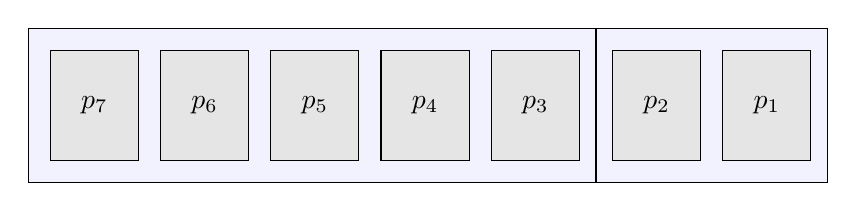
\begin{tikzpicture}[scale=1.4, samples=100]
		
		\filldraw[fill=blue!5!white, draw=black] (0, 0) rectangle (5.15, 1.4);
		\filldraw[fill=gray!20!white, draw=black] (0.2, 0.2) rectangle node{$p_7$} (1.0, 1.2); 
		\filldraw[fill=gray!20!white, draw=black] (1.2, 0.2) rectangle node{$p_6$} (2.0, 1.2); 
		\filldraw[fill=gray!20!white, draw=black] (2.2, 0.2) rectangle node{$p_5$} (3.0, 1.2); 
		\filldraw[fill=gray!20!white, draw=black] (3.2, 0.2) rectangle node{$p_4$} (4.0, 1.2); 
		\filldraw[fill=gray!20!white, draw=black] (4.2, 0.2) rectangle node{$p_3$} (5.0, 1.2); 
		\filldraw[fill=blue!5!white,  draw=black] (5.15,  0) rectangle             (7.25, 1.4);
		\filldraw[fill=gray!20!white, draw=black] (5.3, 0.2) rectangle node{$p_2$} (6.1, 1.2); 
		\filldraw[fill=gray!20!white, draw=black] (6.3, 0.2) rectangle node{$p_1$} (7.1, 1.2);	
		
	\end{tikzpicture}
	
	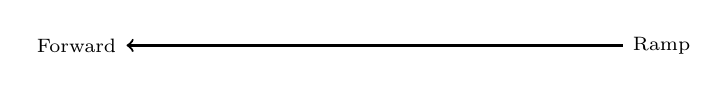
\begin{tikzpicture}[scale=1.4, samples=100]
		\draw[black, thick][<-]  (1, 2.17) node[anchor=east, font=\fontsize{7}{3.5}\selectfont]{Forward} -- (5.5, 2.17) node[anchor=west, font=\fontsize{7}{3.5}\selectfont]{Ramp} ;
	\end{tikzpicture}
	
	\caption{Smaller aircraft layout}
	\label{fig:smaller}
\end{figure}



\begin{figure}[!h]
	\centering
	
	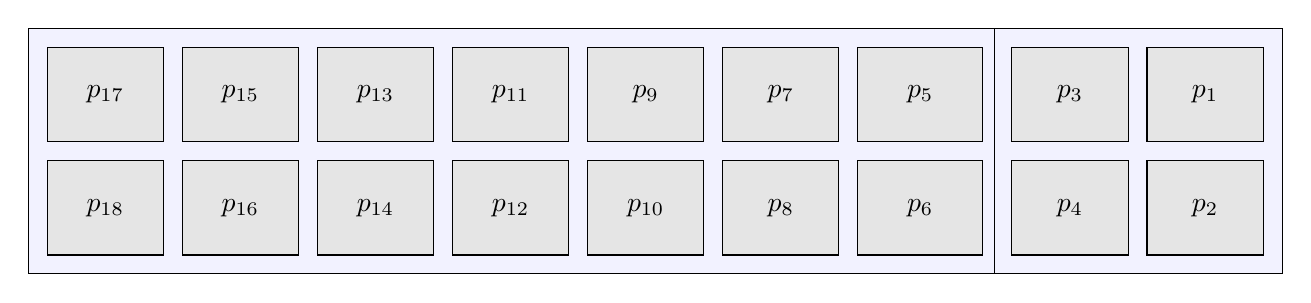
\begin{tikzpicture}[scale=1.2, samples=100]
		
		\filldraw[fill=blue!5!white, draw=black] (0, 0) rectangle (10.23, 2.6);
		
		\filldraw[fill=gray!20!white, draw=black] (0.20, 1.40) rectangle node{$p_{17}$} (1.43, 2.40);
		\filldraw[fill=gray!20!white, draw=black] (0.20, 0.20) rectangle node{$p_{18}$} (1.43, 1.20);
		
		\filldraw[fill=gray!20!white, draw=black] (1.63, 1.40) rectangle node{$p_{15}$} (2.86, 2.40);
		\filldraw[fill=gray!20!white, draw=black] (1.63, 0.20) rectangle node{$p_{16}$} (2.86, 1.20);
		
		\filldraw[fill=gray!20!white, draw=black] (3.06, 1.40) rectangle node{$p_{13}$} (4.29, 2.40);
		\filldraw[fill=gray!20!white, draw=black] (3.06, 0.20) rectangle node{$p_{14}$} (4.29, 1.20);
		
		\filldraw[fill=gray!20!white, draw=black] (4.49, 1.40) rectangle node{$p_{11}$} (5.72, 2.40);
		\filldraw[fill=gray!20!white, draw=black] (4.49, 0.20) rectangle node{$p_{12}$} (5.72, 1.20);
		
		\filldraw[fill=gray!20!white, draw=black] (5.92, 1.40) rectangle node{$p_{9}$} (7.15, 2.40);
		\filldraw[fill=gray!20!white, draw=black] (5.92, 0.20) rectangle node{$p_{10}$} (7.15, 1.20);
		
		\filldraw[fill=gray!20!white, draw=black] (7.35, 1.40) rectangle node{$p_{7}$} (8.58, 2.40);
		\filldraw[fill=gray!20!white, draw=black] (7.35, 0.20) rectangle node{$p_{8}$} (8.58, 1.20);
		
		\filldraw[fill=gray!20!white, draw=black] (8.78, 1.40) rectangle node{$p_{5}$} (10.1, 2.40);
		\filldraw[fill=gray!20!white, draw=black] (8.78, 0.20) rectangle node{$p_{6}$} (10.1, 1.20);
		
		\filldraw[fill=blue!5!white, draw=black] (10.23, 0) rectangle (13.27, 2.6);
		\filldraw[fill=gray!20!white, draw=black] (10.41, 1.40) rectangle node{$p_{3}$} (11.64, 2.40);
		\filldraw[fill=gray!20!white, draw=black] (10.41, 0.20) rectangle node{$p_{4}$} (11.64, 1.20);
		\filldraw[fill=gray!20!white, draw=black] (11.84, 1.40) rectangle node{$p_{1}$} (13.07, 2.40);
		\filldraw[fill=gray!20!white, draw=black] (11.84, 0.20) rectangle node{$p_{2}$} (13.07, 1.20);
		
	\end{tikzpicture}
	
	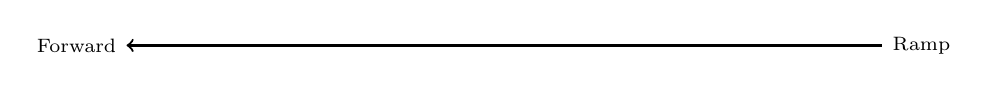
\begin{tikzpicture}[scale=1.2, samples=100]
		\draw[black, thick][<-]  (1, 2.77) node[anchor=east, font=\fontsize{7}{3.5}\selectfont]{Forward} -- (9, 2.77) node[anchor=west, font=\fontsize{7}{3.5}\selectfont]{Ramp} ;
	\end{tikzpicture}
	
	\caption{Larger aircraft layout} \label{fig:larger}
\end{figure}


In both cases, the torque applied to the aircraft must keep its CG in the operational range, which corresponds to a percentage of the {\it Mean Aerodynamic Chord} \footnote{Chord is the distance between the leading and trailing edges of the wing, measured parallel to the normal airflow over the wing. The average length of the chord is known as the {\it Mean Aerodynamic Chord} (MAC).}: $0.556m$ in the smaller aircraft and $1.17m$ in the larger one. See Figure \ref{fig:lateral}.

\begin{figure}[H]
	\centering
	\includegraphics[scale=0.22]{Images/lateral.png}
	\caption{Aircraft longitudinal cut showing red lines as pallets}
	\label{fig:lateral}
\end{figure}


Tables \ref{tab:smaller} and \ref{tab:larger} show the parameters in both cases. {\it CGx} and {\it CGy} refer to the relative distances of pallet centroids (in metres) in relation to the CG of aircraft along both axes. In both aircraft, as the ramps have an inclination of 25 degrees, we made the necessary corrections in {\it CGx}, {\it Weight} and {\it Volume limits} of the corresponding pallets. The monetary costs of both aircraft are also indicated: per unit of distance in flights legs ($c_d$) and per deviation in the CG ($c_g$). It is important to consider that $c_g$ tends to zero as the aircraft attitude tends to level.


\begin{table}[H]
	\centering
	\caption{Smaller aircraft parameters}  \label{tab:smaller}
	\footnotesize
	\begin{tabular}{c | c c c c c c c}
		\toprule
		\textbf{Limits}  & \multicolumn{3}{c}{$Payload$: $26,000kg$} & \multicolumn{4}{c}{$limit^{CG}_{long}$: $0.556m$} \\
		\midrule
		\bf{Pallets} & $p_7$ & $p_6$ & $p_5$ & $p_4$ & $p_3$ & $p_2$ & $p_1$ \\
		\midrule
		{\bf CGx ($m$)}     & -5.10 & -2.70 & -0.30   & 2.10 & 4.50 & 6.25 & 8.39  \\
		\midrule
		{\bf Weight limits ($kg$)}  & 4,500  &  4,500 &  4,500   & 4,500 & 4,500 & 4,000 & 3,500 \\ 
		{\bf Volume limits ($m^3$)} & 13.7  &  13.7 &  13.7   & 13.7 & 13.7 & 8.9 & 6.9 \\ 
		\midrule

		\textbf{Costs}  & \multicolumn{4}{c}{$c_d$: US\$ $1.100/km$ } &	\multicolumn{3}{c}{$c_g = 0.05$} \\

		\bottomrule
	\end{tabular}
	\normalsize 
\end{table}


\begin{table}[H]
	\centering
	\caption{Larger aircraft parameters}  \label{tab:larger}
	\footnotesize
	\begin{tabular}{c | c c c c c c c c c}
		\toprule
		\textbf{Limits}& \multicolumn{3}{c}{$Payload$: $75,000kg$} & \multicolumn{3}{c}{$limit^{CG}_{long}$: $1.170m$} &
		\multicolumn{3}{c}{$limit^{CG}_{lat}$: $0.19m$} \\
		\midrule
		\multirow{2}{*}{\textbf{Pallets}}  & $p_{17}$ & $p_{15}$ & $p_{13}$ & $p_{11}$ & $p_{9}$ & $p_{7}$ & $p_{5}$ & $p_{3}$ & $p_{1}$ \\
		& $p_{18}$ & $p_{16}$ & $p_{14}$ & $p_{12}$ & $p_{10}$ & $p_{8}$ & $p_{6}$ & $p_{4}$ & $p_{2}$ \\
		\midrule 
		\multirow{2}{*}{\textbf{CGx ($m$)}} & -17.57 & -13.17 & -8.77 & -4.40 & 0 & 4.40 & 8.77 & 11.47 & 14.89 \\
		& -17.57 & -13.17 & -8.77 & -4.40 & 0 & 4.40 & 8.77 & 11.47 & 14.89 \\			
		\midrule 
		\multirow{2}{*}{\textbf{CGy ($m$)}}  & 1.32 & 1.32 & 1.32 & 1.32 & 1.32 & 1.32 & 1.32 & 1.32 & 1.32 \\
		& -1.32 & -1.32 & -1.32 & -1.32 & -1.32 & -1.32 & -1.32 & -1.32 & -1.32 \\	
		\midrule
		{\bf Weight limits ($kg$)}      &   4,500   &    4,500  &   4,500   &  4,500    & 4,500     & 4,500     & 4,500     & 4,000    & 3,000   \\
		{\bf Volume limits ($m^3$)}   &   14.8   &   14.8   &  14.8    &  14.8    & 14.8     & 14.8     & 14.8     & 10.0    & 7.0 \\	
		\midrule	

		\textbf{Costs}  & \multicolumn{5}{c}{ $c_d$: US\$ $4.900/km$ } &	\multicolumn{4}{c}{$c_g = 0.05$} \\

		\bottomrule
	\end{tabular}
	\normalsize 
\end{table}

We also make the following assumptions:
\begin{itemize}
	\item on each pallet, the items are distributed in such a way that their CG coincides with the centroid of the pallet;
	\item the CG of the payload must be at a maximum longitudinal distance of $limit^{CG}_{long}$ from the CG of the aircraft;
	\item in the larger aircraft, the CG of the payload must be at a maximum lateral distance of $limit^{CG}_{lat}$ from the CG of the aircraft;
	\item in the larger aircraft, pallets are distributed in two identical rows (with odd and even indices, respectively), and their centroids are at a distance $d^{CG}_{pallet}$ from the center-line of the aircraft.
\end{itemize}




\subsection{Problem summary}

\newcolumntype{M}{>{\raggedright}p{0.03\textwidth}}
\newcolumntype{T}{>{\raggedright\arraybackslash}p{0.9\textwidth}}

\bgroup
\def\arraystretch{1.2}
\begin{table}[H]
	\centering
	\small
	\begin{tabular}{MT}
		&Informally, ACLP+RPDP can be summarised as follows:\\
		\midrule
		max &  (items score sum) / (tour cost) of picked up and delivered items at each node on a tour  \\
		\midrule
s.t.    & Along a tour, the set of unvisited nodes is updated. \\
		& In each node, an item may be included in at most one pallet.\\		
		& In each node, consolidated items are composed of items with the same destination. \\
		& Weight, volume and score of a consolidated item are the corresponding sum of their components.\\
		& Consolidated items remain on board until their destinations.\\	
		& Consolidated items can only be included in the same pallet if their destinations are the same.\\
		& Only items destined to the remaining nodes can be loaded.  \\
		& The lateral and longitudinal torques must be within the operational range of the aircraft.\\
		& Weight and volume limitations of the pallets must be respected.\\
		& The total weight must be less than the aircraft payload or the total pallet capacity, whichever is the lowest.\\	
		\midrule
	\end{tabular}
	\normalsize
\end{table}
\egroup 



\section{The mathematical modeling}
\label{sec4}

Given the assumptions, scenarios and parameters described in the previous section, we are ready to present the mathematical modeling of ACLP+RPDP, which is one of the contributions of our work.

Let $L = \{ l_0, l_1, \ldots, l_K \}$ be the set of $K+1$ nodes (or destinations), where $l_0$ is the origin and end of a tour. Let $d(l_i,l_j)$ be the distance from $l_i$ to $l_j$, where $0 \leq i,j \leq K$. By definition, $d(l_i,l_i)=0$. Let $L_k$ be the set of remaining nodes when the aircraft is in $l_k$, $0 \leq k \leq K$. Therefore, $L_0=L$ and $L_K = \{ l_0 \}$.

Let $C=\{c_{ij}\}$ be the cost matrix of flights, where $c_{ij} = c_d*d(l_i,l_j), 0 \leq i,j \leq K$.

Let $S_K = \{s: \{1, \dots, K\} \rightarrow \{1, \dots, K\} \}$ be the set of $K!$ permutations, which correspond to all possible tours (or itineraries) that have $l_0$ as origin and end, passing through the others $K$ nodes.

Let $M = \{p_1, p_2, \ldots, p_m \}$ the set of $m$ pallets. Each pallet $p_i$, $1 \leq i \leq m$, has weight capacity $p_i.w$, volume capacity $p_i.v$, pallet destinations $p_i.to[k]$, $0 \leq k \leq K$, and distance to the CG of aircraft $p_i.d$. $p_i.to[k]$ denotes that pallet $p_i$ may assume a different destination in each node $k$.

Let $N_k = \{t^k_1, t^k_2, \ldots, t^k_{n_k} \}$ be the set of $n_k$ items to be loaded in node $l_k$, $0 \leq k \leq K$. Each item $t^k_j$, $1 \leq j \leq n_k$, has score $t^k_j.s$, weight $t^k_j.w$, volume $t^k_j.v$, and destination $t^k_j.to \in L_k$. Let $N = \bigcup_{0 \leq k \leq K} N_k$ be the set of items of all nodes along a tour.

Let $Q_k = \{a^k_1, a^k_2, \ldots, a^k_{m_k} \}$ be the set of consolidated items loaded in $m_k \leq m$ pallets when the aircraft arrives at node $l_k$, with $0 \leq k \leq K$. $a^k_i$, $1 \leq i \leq m_k$, is the group of picked-up items that were allocated on pallet $p_i$ in some of the previous nodes. $a^k_i$ has total weight $a^k_i.w$, total volume $a^k_i.v$, and destination $a^k_i.to \in L_k \cup \{l_k\}$. If $a^k_i.to = l_k$, then $a^k_i$ is unloaded, and $p_i$ will be available for reloading; otherwise, $a^k_i$ remains on the aircraft, eventually in another pallet, and with items of $N_k$ having the same destination.

Let $X_{ij}^k$ and $Y_{iq}^k$ be binary variables, where $0 \leq k \leq K$, $1 \leq j \leq n_k$, $1 \leq i \leq m$ and $1 \leq q \leq m_k$. $X_{ij}^k = 1$ if $t_j^k$ is assigned to $p_i$ in node $l_k$, and 0 otherwise. $Y_{iq}^k = 1$ if $a_q^k$ is assigned to $p_i$ in node $l_k$, and 0 otherwise. By definition, $Y_{iq}^0=0$. Allocations of items or consolidated items to pallets in node $l_k$ can be seen as a bipartite graph $G_k(V_k, E_k)$, where $V_k = M \cup N_k \cup Q_k$, $E_k = E^N_k \cup E^Q_k$, $(p_i, t_j^k) \in E^N_k$ if $X_{ij}^k = 1$, and $(p_i, a_q^k) \in E^Q_k$ if $Y_{iq}^k = 1$.

The mathematical modeling of this problem is described in the equations below.


\begin{equation} \label{eq:maxf}
	\max_{\pi \in S_K} f_\pi(\tilde{s},\tilde{c})
\end{equation}

\begin{equation} \label{eq:scores}
	\tilde{s} = \sum_{k=0}^{K} \sum_{i=1}^{m} \sum_{j=1}^{n_k} X_{ij}^k \times t_j^k.s
\end{equation}

\begin{equation} \label{eq:costs}
	\tilde{c} = c_{0,\pi(1)}\times(1+c_g\times|\epsilon_0|) + \sum_{k=1}^{K-1} [ c_{\pi(k), \pi(k+1)}\times(1+c_g\times|\epsilon_k|) ] + c_{\pi(K),0}\times(1+c_g\times|\epsilon_K|)
\end{equation}

\begin{equation} \label{eq:maxW}
	maxW = \min(Payload, \sum_{i=1}^{m}p_i.w)
\end{equation}

\begin{equation} \label{eq:tau}
\tau_k = \sum_{i=1}^{m}[ p_i.d \times (\sum_{j=1}^{n_k} X_{ij}^k \times t_j^k.w +  \sum_{q=1}^{m} Y_{iq}^k \times a_q^k.w)];\ k \in \{0, 1, \ldots, K\}
\end{equation}

\begin{equation} \label{eq:eps}
\epsilon_k = \frac{\tau_k}{maxW \times limit^{CG}_{long}};\ k \in \{0, 1, \ldots, K\}
\end{equation}

\begin{equation} \label{eq:pdp11}
	L_0 = L; L_{k} = L_{k-1} - \{l_{\pi(k)}\}; \ k \in \{1, 2, \ldots, K\}
\end{equation}

\begin{equation} \label{eq:pdp13}
	Y^0_{iq} = 0; a^0_i.w = 0; a^0_i.v = 0; a^0_i.to = -1;\ i,q \in \{1, 2, \ldots, m\}
\end{equation}

\begin{equation} \label{eq:pdp12}
	X_{ij}^k = 0 \ \mbox{if} \ t_j^k.to \notin L_k; \ i \in \{1, 2, \ldots, m\}; \ j \in \{1, 2, \ldots, n_k\}; \ k \in \{1,2, \ldots, K\}
\end{equation}

\begin{equation} \label{eq:pdp9}
	Y_{iq}^k = 0 \ \mbox{if} \ a_i^k.to \notin L_k; \ i \in \{1, 2, \ldots, m\}; \ q \in \{1, 2, \ldots, m_k\}; \ k \in \{ 1, 2, \ldots, K\}
\end{equation}

\begin{equation} \label{eq:cons2}
	a_i^{\pi(k+1)}.w = \sum_{j=1}^{n_k} X_{ij}^{\pi(k)} \times t_j^{\pi(k)}.w + \sum_{q=1}^{m_k} Y_{iq}^{\pi(k)} \times a_q^{\pi(k)}.w;  \ i \in \{1, 2, \ldots, m_k\}; k \in \{0, 1, \ldots, K-1\}
\end{equation}

\begin{equation} \label{eq:cons3}
	a_i^{\pi(k+1)}.v = \sum_{j=1}^{n_k} X_{ij}^{\pi(k)} \times t_j^{\pi(k)}.v + \sum_{q=1}^{m_k} Y_{iq}^{\pi(k)} \times a_q^{\pi(k)}.v;  \ i \in \{1, 2, \ldots, m_k\}; k \in \{0, 1, \ldots, K-1\}
\end{equation}

\begin{equation} \label{eq:cons5}
	a_i^{\pi(k+1)}.to = t^{\pi(k)}_j.to  \ \mbox{if} \ X^{\pi(k)}_{ij} = 1  \ \mbox{and} \ t^{\pi(k)}_j.to \in L_{k+1};  \ i \in \{1, 2, \ldots, m_k\}; \ j \in \{1, 2, \ldots, n_k\}; \ k \in \{0,1, \ldots, K-1\}
\end{equation}

\begin{equation} \label{eq:LatIt}
	LatIt_k = \sum_{i=1}^{m} \sum_{j=1}^{n_k} ( X_{ij}^k \times t_j^k.w \times (i\%2) - X_{ij}^k \times t_j^k.w \times (i+1)\%2 ); \ k \in \{0, 1, \ldots, K\}
\end{equation}

\begin{equation} \label{eq:LatCons}
	LatCons_k =  \sum_{i=1}^{m} \sum_{q=1}^{m_k}  ( Y_{iq}^k \times a_q^k.w \times (i\%2) - Y_{iq}^k \times a_q^k.w \times (i+1)\%2); \ k \in \{0, 1, \ldots, K\}
\end{equation}

\begin{equation} \label{eq:torqlat}
	s.t.: d^{CG}_{pallet} \times | LatIt_k + LatCons_k | \leq  \sum_{i=1}^{m}p_i.w \times limit^{CG}_{lat}; \ k \in \{0, 1, \ldots, K\}
\end{equation}

\begin{equation} \label{eq:torqlong}
	s.t.: |\tau_k| \leq maxW \times limit^{CG}_{long};\ k \in \{0, 1, \ldots, K\}
\end{equation}

\begin{equation} \label{eq:payload}
	s.t.: \sum_{i=1}^{m} (\sum_{j=1}^{n_k} X_{ij}^k \times t_j^k.w + \sum_{q=1}^{m_k} Y_{iq}^k \times a_q^k.w ) \leq maxW; \ k \in \{0, 1, \ldots, K\}
\end{equation}

\begin{equation} \label{eq:app2}
	s.t.: \sum_{j=1}^{n_k} X_{ij}^k \times t_j^k.w + \sum_{q=1}^{m_k} Y_{iq}^k \times a_q^k.w  \leq p_i.w; \ i \in \{1, 2, \ldots, m_k\}; \ k \in \{0, 1, \ldots, K\}
\end{equation}

\begin{equation} \label{eq:app3}
	s.t.: \sum_{j=1}^{n_k} X_{ij}^k \times t_j^k.v + \sum_{q=1}^{m_k} Y_{iq}^k \times a_q^k.v  \leq\ p_i.v; \ i \in \{1, 2, \ldots, m_k\}; \ k \in \{0, 1, \ldots, K\}
\end{equation}

\begin{equation} \label{eq:app4}
	s.t.: \sum_{i=1}^{m} X_{ij}^k \leq 1; \ j \in \{1, 2, \ldots, n_k\}; \ k \in \{0, 1, \ldots, K\}
\end{equation}

\begin{equation} \label{eq:app5}
	s.t.:  Y_{iq}^k = 1 \ \mbox{if} \ a^k_q.to \in L_k; \ q \in \{1, 2, \ldots, m_k\}; \ k \in \{0, 1, \ldots, K\}
\end{equation}

\begin{equation} \label{eq:pdp8}
	s.t.: p_i.to[k] = t^k_j.to\ \mbox{if} \ X_{ij}^k = 1; \ i \in \{1, 2, \ldots, m\}; \ j \in \{1, 2, \ldots, n_k\}; \ k \in \{1, 2, \ldots, K\}
\end{equation}

\begin{equation} \label{eq:pdp2}
	s.t.:  p_i.to[k] = a^k_q.to\ \mbox{if} \ Y_{iq}^k = 1; \ i \in \{1, 2, \ldots, m\};\ q \in \{1, 2, \ldots, m_k\}; \ k \in \{1, 2, \ldots, K\}
\end{equation}


The objective of this problem is to find a permutation $\pi \in S_K$\/ that maximizes the function $f_\pi(\tilde{s},\tilde{c})$ \ref{eq:maxf}. In this way, the tour plan will be $l_0, l_{\pi(1)}, \ldots, l_{\pi(K)}, l_0$. $\tilde{s}$\/ is the total score of transported items \ref{eq:scores} and  $\tilde{c}$\/ is the total cost of fuel consumed \ref{eq:costs}. As can be seen, $\tilde{c}$\/ corresponds to the fuel consumption due to the flights carried out and the CG deviation of the transported cargo. Throughout this work, for simplicity, we use $f=\tilde{s}/\tilde{c}$.

The maximum load will be the minimum between the payload and the capacity supported by the pallets \ref{eq:maxW}. Considering the maximum longitudinal distance allowed for the CG, all torques \ref{eq:tau} and deviations \ref{eq:eps} are calculated.

For each step of the tour, the set of unvisited nodes is updated \ref{eq:pdp11}. Although there are no items consolidated at the beginning of the tour, we defined these variables for ease of notation \ref{eq:pdp13}. Items destined outside the rest of the tour will not be loaded (\ref{eq:pdp12} and \ref{eq:pdp9}).

Consolidated items appear when there are items on the pallets that will not be unloaded on the next node. Its weights \ref{eq:cons2} and volumes \ref{eq:cons3} correspond to all the items that were on the pallet, since all these items have the same destination. On subsequent nodes, consolidated items can be allocated with other items of same destination \ref{eq:cons5}.

Equations \ref{eq:LatIt} and \ref{eq:LatCons} respectively, are applied only to the larger aircraft, and calculate the lateral torques of items and consolidated items loaded in both rows of pallets, whose constraint is described in \ref{eq:torqlat}. Similarly, \ref{eq:torqlong} is the longitudinal torque constraint, which is applied to both aircraft sizes.

The weight limitation of the aircraft must be respected \ref{eq:payload}. The sum of weights \ref{eq:app2} and volumes \ref{eq:app3} in each pallet must not exceed its capacity. Each item is associated with a pallet at most \ref{eq:app4}.

Consolidated items remain on board \ref{eq:app5} until their destinations. At each node, an item (\ref{eq:pdp8}) and a consolidated item (\ref{eq:pdp2}) must only be allocated to a pallet if the destinations are the same.



\section{Resolution strategy}
\label{sec5}

Once the assumptions of this work and the mathematical modeling of the problem are presented, it is easy to see that ACLP+RPDP is NP-hard. In a similar way to Lurkin and Schyns \cite[p. 6]{LurkinSchyns2015}, consider the simple case where $K=1$\/ (one leg), $m=2$ (two pallets around the aircraft CG), $2n$\/ sufficiently light items with same scores in $l_0$, and no items in $l_1$. Under these conditions, through polynomial reductions for the {\it Set-Partition Problem}, it is possible to demonstrate that the decision problem associated with ACLP+RPDP is NP-complete.

Real cases are more complex as they have hundreds of different items in each node and involve four intractable sub-problems: APP, WBP, PDP and TSP. Through the mathematical modeling presented in the previous section, we verify that {\it Mixed-Integer Programming}\/ (MIP) is not able to solve these cases in feasible time. Thus, it is necessary to adopt some strategy to find a viable solution, not necessarily optimal, that seeks to maximize the objective function $f$.

Our strategy is based on the fact that, in real cases, $K$\/ is usually small. Specifically, we will consider $K \leq 6$\/ throughout this work, which is a higher value than usual in {\it Brazilian Air Force} missions. As a result, if we have fast node-by-node solutions that allow us to construct a complete tour, we will be able to test all possible $K!$\/ tours and thus select the one that provides the best value for the $f$\/ function.

On the other hand, our tactic will be, at each shipping node, to predefine the destinations of the pallets at that node. In this way, we will reserve a number of pallets proportional to the volume demanded by each destination at the shipping node. We could have used another criterion, but it was observed in the experiments that volume is more constrictive in airlift. Once the destinations of the pallets are defined, we will use heuristics and a MIP solver to find the best possible node-by-node solutions. This strategy is summarized in Algorithm \ref{alg:main}.


\begin{algorithm}[H]
	\caption{Main procedure}  \label{alg:main}
	\begin{algorithmic}[1]
		
		\Procedure{$ACLP+RPDP$}{$scenario,\ volume$}
		
		\State Let $L, M, C$ be according to $scenario$ \label{main:LMC} \Comment{Nodes, pallets and costs}
		\State $N \gets ItemsGeneration(scenario,\ volume)$ \label{main:items} \Comment{Items available for shipment}
		\For {each $method$} \Comment{$method$ is a MIP solver or a heuristic}
			\For {each $\pi \in S_K$} \label{main:loop1} \Comment{$\pi$ is a permutation of the nodes}
				\State $f_{\pi} \gets SolveTour(\pi, L, M, C, N, method )$ \Comment{A solution to the permutation $\pi$} \label{main:method}
			\EndFor \label{main:loop2}
			\State $answer[scenario,volume,method] \gets \max f$ \label{main:f} \Comment{Best result among all permutations}
		\EndFor
		\Return $answer$
		
		\EndProcedure
		
	\end{algorithmic}
\end{algorithm}


In this algorithm, there are six values for the $scenario$\/ parameter, according to Table \ref{tab:scenarios}, which defines $K$, the sets of nodes, the aircraft, the pallets and the costs from Tables \ref{tab:smaller} or \ref{tab:larger} that will be used (line \ref{main:LMC}).

The parameter $volume$\/ is a value greater than 1, which corresponds, at each node $l_k$, to the ratio between the sum of the volumes of the items ($\sum_{j=1}^{n_k} t^k_j.v$) and the load capacity of the pallets ($\sum_{i=1}^{m} p_i.v$). This parameter is passed to $ItemsGeneration$\/ (line \ref{main:items}), responsible for creating the items to be shipped, which will be presented in the next section (Algorithm \ref{alg:itemsgen}).

$method$\/ corresponds to a MIP solver or a heuristic that we will present in subsection \ref{methods}. The loop of lines \ref{main:loop1}-\ref{main:loop2} goes through all permutations $\pi$, where the node-by-node resolutions are performed by $SolveTour$, whose result is stored in $f_{\pi}$. The best result among all $K!$\/ tours will be the answer for $scenario$, $volume$\/ and $method$\/ (line \ref{main:f}).


\vspace{2.0mm}
\begin{table}[H]
	\centering
	\caption{Testing scenarios}  \label{tab:scenarios}
	\begin{tabular}{c c c c }
		\toprule
		{\bf Scenario} & {$K$} & {$L$} & {\bf Aircraft} \\		
		\midrule
		1 & 2    & \{$l_0$, $l_1$, $l_2$\}                                 & smaller \\
		2 & 2    & \{$l_0$, $l_1$, $l_2$\}                                 & larger  \\
		3 & 3    & \{$l_0$, $l_1$, $l_2$, $l_3$\}                          & larger  \\
		4 & 4    & \{$l_0$, $l_1$, $l_2$, $l_3$, $l_4$\}                   & larger  \\
		5 & 5    & \{$l_0$, $l_1$, $l_2$, $l_3$, $l_4$, $l_5$\}            & larger  \\
		6 & 6    & \{$l_0$, $l_1$, $l_2$, $l_3$, $l_4$, $l_5$, $l_6$\}     & larger  \\
		\bottomrule
	\end{tabular}
\end{table}

Next, we will present two subsections: in the first we explain how $SolveTour$ is executed, while in the second we will present the heuristic developed for node-by-node resolutions.


\subsection{SolveTour algorithm}
\label{tour}

In addition to the set of nodes, pallets, costs and items, $SolveTour$, described in Algorithm \ref{alg:tour}, receives the parameter $method$, which corresponds to a MIP solver or a heuristic for solving the node-by-node problems, and the parameter $\pi$, which is a permutation that defines the order of visits in this tour.

As we mentioned in the previous section, all tours start and end at $l_0$\/ (lines \ref{tour:pi1}-\ref{tour:pi2}). After initializing the score and cost values (lines \ref{tour:score}-\ref{tour:cost}), there is a loop for the $K+1$\/ flights (lines \ref{tour:loop1}-\ref{tour:loop2}). Initially we set pallets destination as $-1$\/ (line \ref{tour:-1}). When the aircraft is at node $l_0$, the initial graph $G_1$\/ is empty because it has no consolidated items \ref{tour:g11}. Otherwise, the set $L_k$\/ of remaining nodes is updated (line \ref{tour:lk1}), and $UpdateConsolidated$\/ (line \ref{tour:dest}) returns the set of consolidated items that have not yet reached their destination and remain on board, rearranging them on the pallets to minimize CG deviation. This allocation is stored in graph $G_1$\/ (line \ref{tour:g12}).

In the context of this work, we know that $m>K$, once the aircraft has $7$\/ or $18$\/ pallets and $K\leq 6$, allowing there to be at least one pallet for each node to be visited. $SetPalletsDestinations$\/ (line \ref{tour:dest2}) presets the destination of each pallet based on the volume demands of the current node, without changing the pallets destination with consolidated items.

Finally, $SolveNode$\/ includes the edges corresponding to the items shipped at the current node, returning the graph $G_2$\/ (line \ref{tour:node}). The score and the CG deviation of this graph are calculated (line \ref{tour:analyse}) and accumulated (lines \ref{tour:score2}-\ref{tour:cost2}), allowing the final result of this tour (line \ref{tour:f}).

\begin{algorithm}[H]
	\caption{Procedure to solve tour $\pi$ with $method$ (MPI solver or heuristic)}  \label{alg:tour}
	\begin{algorithmic}[1]
		
		\Procedure{$SolveTour$}{$\pi, L, M, C, N, method$}
		
		\State $\pi(0) \gets 0$ \label{tour:pi1} \Comment{The first node is the base}
		\State $\pi(K+1) \gets 0$ \label{tour:pi2} \Comment{The last node is also the base}
		\State $score \gets 0$ \label{tour:score}
		\State $cost \gets 0$ \label{tour:cost}
		\For {$k\gets0$ to $K$} \label{tour:loop1}		
			\For{$i \gets 1$ to $m$}
				\State $p_i.to[k] \gets -1$ \label{tour:-1} \Comment{Pallet destination unset}
			\EndFor	
			\If {$k = 0$}
				\State $L_0 \gets L$
				\State Let $G_1(M \cup N_0, \varnothing)$ \label{tour:g11}
			\Else
				\State $L_k \gets L_k - \pi(k)$  \label{tour:lk1}	\Comment{$\pi(k)$ is the node $k$ from tour $\pi$}		
				\State $Q_{\pi(k)}, E^Q_{\pi(k)}, M \gets UpdateConsolidated(\pi(k))$ \label{tour:dest}			
				\State Let $G_1(M \cup N_{\pi(k)} \cup Q_{\pi(k)}, E^Q_{\pi(k)})$ \label{tour:g12}
			\EndIf  \label{tour:lk2}	
			\State $M \gets SetPalletsDestinations( \pi(k) )$ \label{tour:dest2}		
			\State $G_2 \gets SolveNode(method, \pi(k), G_1)$ \label{tour:node}
			\State $s, \epsilon \gets ScoreAndDeviation(\pi(k), G_2)$ \label{tour:analyse}
			\State $score \gets score + s$ \label{tour:score2}
			\State $cost \gets cost + c_{\pi(k),\pi(k+1)} * (1 + c_g * |\epsilon|)$ \label{tour:cost2} 
		\EndFor  \label{tour:loop2}
		\Return $score / cost$ \label{tour:f}
		
		\EndProcedure
		
	\end{algorithmic}
\end{algorithm}

$UpdateConsolidated$, described in Algorithm \ref{alg:cons}, finds the best allocation for the consolidated items that remain on board. Initially, the set $Q$\/ is created, with the consolidated items that did not reach their destination (lines \ref{cons:remain1}-\ref{cons:remain2}). Then $MinCGDeviation$\/ (line \ref{cons:minCG}) is run through a MIP solver with the equations \ref{eq:torque}, \ref{eq:embarked} and \ref {eq:one}, to relocate the consolidated items on the pallets minimizing torque and ensuring that they all remain on board, one on each pallet. As there are few variables, the MIP solver returns an allocation $E^Q_k$\/ very quickly. Finally, the destination of each pallet with consolidated items is updated (lines \ref{cons:Ybegin}-\ref{cons:Yend}).

\begin{algorithm}[H]
	\caption{Procedure to update consolidated items that remain boarded on node $k$}  \label{alg:cons}
	\begin{algorithmic}[1]
		
		\Procedure{$UpdateConsolidated$}{$k$}
		
		\State Let $Q_k  = \{ a^k_1, a^k_2, \ldots, a^k_{m_k} \}$ 
		\State $Q \gets \varnothing$ \label{cons:remain1}
		\For{$q\gets1$ to $m_k$} 
			\If {$a_q^k.to \in L_k$} 
				\State $Q \gets Q \cup \{a_q^k\}$
			\EndIf
		\EndFor	 
		\State $m_k \gets |Q|$ \label{cons:remain2}
		\State $E^Q_k \gets MinCGDeviation(k, Q)$ \label{cons:minCG}
		\For{$i \gets 1$ to $m$} \label{cons:Ybegin}
			\For{$q \gets 1$ to $m_k$}
				\If{$(p_i, a_q^k) \in E^Q_k$} 
					\State $p_i.to[k] \gets a_q^k.to$
				\EndIf
			\EndFor		
		\EndFor \label{cons:Yend}
		\Return $Q, E^Q_k, M$
		\EndProcedure
	\end{algorithmic}
\end{algorithm}



\begin{equation} \label{eq:torque}
	\mbox{minimize}\ | \sum_{i=1}^{m} \sum_{q=1}^{m_k} Y^k_{iq} \times p_i.d \times a_q^k.w |,\ \mbox{where}\ Q  = \{ a^k_1, a^k_2, \ldots, a^k_{m_k} \} 
\end{equation}

\begin{equation} \label{eq:embarked}
	s.t.: \sum_{i=1}^{m} Y^k_{iq} = 1;\ q \in \{1,2,\ldots,m_k\}
\end{equation}

\begin{equation} \label{eq:one}
	s.t.: \sum_{q=1}^{m_k} Y^k_{iq} \leq 1;\ i \in \{1,2,\ldots,m\}
\end{equation}


$SetPalletsDestinations$, which set pallets destination not yet defined, is described in Algorithm \ref{alg:dest}. The vectors $vol[0..K]$\/ and $PalCons[0..K]$\/ store the total volume of items and the number of pallets with consolidated items destined for each node, respectively (lines \ref{dest:vector1}-\ref{dest:vector2}). The destinations of each pallet are defined proportionally to the volume of items, regarding the pallets with consolidated items (lines \ref{dest:propor1}-\ref{dest:propor2}). The node with the maximum volume demand defines the destination of any remaining pallets (lines \ref{dest:max1}-\ref{dest:max2}).


\begin{algorithm}[H]
	\caption{Procedure to set pallets destinations based on the items to be embarked on node $k$}  \label{alg:dest}
	\begin{algorithmic}[1]
		
		\Procedure{$SetPalletsDestinations$}{$k$}
		
		\For{$x \gets 0$ to $K$} \label{dest:vector1}
			\State $vol[x] \gets 0$ 
			\State $PalCons[x]  \gets 0$
		\EndFor
		\State $max \gets 0$ \label{dest:max}
		\State $total \gets 0$ 
		\For{$j \gets 1$ to $n_k$}
			\State $d \gets t_j^k.to$
			\If {$d \in L_k$} 
				\State $vol[d] \gets vol[d] + t_j^k.v$ 
				\State $total \gets total + t_j^k.v$ 
				\If {$vol[d] > vol[max]$}
					\State $max \gets d$ 
				\EndIf
			\EndIf
		\EndFor
		\For{$q \gets 1$ to $m_k$}
			\State $d \gets a_q^k.to$
			\State $PalCons[d] \gets PalCons[d]+1$
			\If {$d \in L_k$} 
				\State $vol[d] \gets vol[d] + a_q^k.v$
				\State $total \gets total + a_q^k.v$ 
				\If {$vol[d] > vol[max]$}
					\State $max \gets d$ 
				\EndIf
			\EndIf
		\EndFor \label{dest:vector2}
		\For{$x \gets 0$ to $K$} \label{dest:propor1}
			\If {$vol[x] \neq 0$}
				\State $quant \gets \max \{1, \lfloor{ m \times vol[x]/total}\rfloor \}-PalCons[x]$  \Comment{Number of pallets needed}
				\State $np \gets 0$
				\For{$i \gets 1$ to $m$}
				
					\If{$np = quant$}
						\State ${\bf break}$
					\EndIf
					\If{$p_i.to[k] = -1$}              \Comment{Pallet destination in node $k$ was unset}
						\State $p_i.to[k] \gets x$
						\State $np \gets np + 1$
					\EndIf
				\EndFor
			\EndIf 
		\EndFor \label{dest:propor2}
		\For{$i \gets 1$ to $m$} \label{dest:max1}
			\If{$p_i.to[k] = -1$}
				\State $p_i.to[k] \gets max$
			\EndIf
		\EndFor \label{dest:max2}
		\Return $M$
		\EndProcedure
	\end{algorithmic}
\end{algorithm}


$ScoreAndDeviation$\/ is described in Algorithm \ref{alg:eval}, which evaluates the allocation graph generated by $SolveNode$, returning the corresponding score and CG deviation. It consists of a loop that goes through all the pallets (lines \ref{eval:loop1}-\ref{eval:loop2}), accumulating the scores (lines \ref{eval:score1}-\ref{eval:score2} ) and the torques (lines \ref{eval:eps1}-\ref{eval:eps2}) of the shipped items, allowing the final calculation of the CG deviation (lines \ref{eval:torque1}-\ref{eval:torque2}).


\begin{algorithm}[H]
	\caption{Procedure to calculate the solution score and the relative torque deviation on node $k$}  \label{alg:eval}
	\begin{algorithmic}[1]
		
		\Procedure{$ScoreAndDeviation$}{$k,\ G$}
		
		\State Let $G(V_k, E^N_k \cup E^Q_k)$
		\State Let $X_{ij}^k = 1$ if $(p_i, t_j^k) \in E^N_k$, $1 \leq i \leq m$, $1 \leq j \leq n_k$
		\State Let $Y_{iq}^k = 1$ if $(p_i, a_q^k) \in E^Q_k$, $1 \leq i \leq m$, $1 \leq q \leq m_k$
		\State $s \gets 0$
		\State $\epsilon \gets 0$
		\State $weight \gets 0$
		\For{$i \gets 1$ to $m$}	\label{eval:loop1}
			\State $weight \gets weight + p_i.w$		
			\For{$j \gets 1$ to $n_k$}
				\If{$X_{ij}^k = 1$}
					\State $s \gets s + t_{ij}^k.s$ \label{eval:score1}
					\State $\epsilon \gets \epsilon + t_{ij}^k.w * p_i.d$ \label{eval:eps1}
				\EndIf
			\EndFor				
			\For{$q \gets 1$ to $m_k$}
				\If{$Y_{iq}^k = 1$}
					\State $s \gets s + a_{iq}^k.s$   \label{eval:score2}
					\State $\epsilon \gets \epsilon + a_{iq}^k.w * p_i.d$  \label{eval:eps2}
				\EndIf
			\EndFor	   \label{eval:loop2}
		\EndFor
		\State $maxWeight \gets \min(Payload, weight)$ \label{eval:torque1}
		\State $maxTorque \gets maxWeight \times limit^{CG}_{long}$
		\State $\epsilon \gets \epsilon/maxTorque$ \label{eval:torque2}
		\Return $s,\ \epsilon$
		\EndProcedure
			
	\end{algorithmic}
\end{algorithm}


\subsection{Node-by-node solutions}
\label{methods}


In this subsection we present two implementations of $SolveNode(method,\ k,\ G)$, where  $k$\/ is the index of the current node and $G$\/ is the allocation graph of the consolidated items that remain on board at node $l_k$. These implementations correspond to the two possible values of the $method$\/ parameter: $MPI$\/ (a solver) or $Shims$\/ (a heuristic).


\subsubsection{MIP solver}
\label{solver}

To find a viable solution for ACLP+RPDP, the strategy adopted in $SolveTour$\/ previously defines the values of some variables. Concretely, all permutations between the nodes are tested, the set of nodes to be visited is updated, the consolidated items that remain on board are reallocated to minimize the CG deviation, and the pallets destination is determined according to the volume of items available for shipment. In this way, the mathematical modeling for $SolveNode(MIP,\ k,\ G)$\/ becomes simpler, which finds an allocation of available items in node $l_k$\/ using previously defined values of $L_k$, $p_i.to[k]$, $Y^k_{iq}$\/ and $a^k_q$. 

This simplified modeling is described in the equations \ref{eq:newf} to \ref{eq:lastnew}, which maximizes the score of the $t^k_j$\/ items to be shipped, maintaining load balancing. The variables $X^k_{ij}$\/ define the set of edges $E^N_k$, which will be added to the graph $G$.


\begin{equation} \label{eq:newf}
	\max f_s = \sum_{i=1}^{m} \sum_{j=1}^{n_k} X_{ij}^k \times t_j^k.s
\end{equation}

\begin{equation} 
	maxW = \min(Payload, \sum_{i=1}^{m}p_i.w)
\end{equation}

\begin{equation} 
	\epsilon_k = \sum_{i=1}^{m}[ p_i.d \times (\sum_{j=1}^{n_k} X_{ij}^k \times t_j^k.w +  \sum_{q=1}^{m} Y_{iq}^k \times a_q^k.w)]/(maxW \times limit^{CG}_{long})
\end{equation}

\begin{equation}
	X_{ij}^k = 0 \ \mbox{if} \ t_j^k.to \notin L_k; \ i \in \{1, 2, \ldots, m\}; \ j \in \{1, 2, \ldots, n_k\}
\end{equation}

\begin{equation} 
	LatIt_k = \sum_{i=1}^{m} \sum_{j=1}^{n_k} ( X_{ij}^k \times t_j^k.w \times (i\%2) - X_{ij}^k \times t_j^k.w \times (i+1)\%2 )
\end{equation}

\begin{equation} 
	LatCons_k =  \sum_{i=1}^{m} \sum_{q=1}^{m_k}  ( Y_{iq}^k \times a_q^k.w \times (i\%2) - Y_{iq}^k \times a_q^k.w \times (i+1)\%2)
\end{equation}

\begin{equation} 
	s.t.: d^{CG}_{pallet} \times | LatIt_k + LatCons_k | \leq  \sum_{i=1}^{m}p_i.w \times limit^{CG}_{lat}
\end{equation}

\begin{equation}
	s.t.: |\tau_k| \leq maxW \times limit^{CG}_{long}
\end{equation}

\begin{equation} 
	s.t.: \sum_{i=1}^{m} (\sum_{j=1}^{n_k} X_{ij}^k \times t_j^k.w + \sum_{q=1}^{m_k} Y_{iq}^k \times a_q^k.w ) \leq maxW
\end{equation}

\begin{equation} 
	s.t.: \sum_{j=1}^{n_k} X_{ij}^k \times t_j^k.w + \sum_{q=1}^{m_k} Y_{iq}^k \times a_q^k.w  \leq p_i.w; \ i \in \{1, 2, \ldots, m_k\}
\end{equation}

\begin{equation} 
	s.t.: \sum_{j=1}^{n_k} X_{ij}^k \times t_j^k.v + \sum_{q=1}^{m_k} Y_{iq}^k \times a_q^k.v  \leq\ p_i.v; \ i \in \{1, 2, \ldots, m_k\}
\end{equation}

\begin{equation} 
	s.t.: \sum_{i=1}^{m} X_{ij}^k \leq 1; \ j \in \{1, 2, \ldots, n_k\}
\end{equation}

\begin{equation} \label{eq:lastnew}
	s.t.: p_i.to[k] = t^k_j.to\ \mbox{if} \ X_{ij}^k = 1; \ i \in \{1, 2, \ldots, m\}; \ j \in \{1, 2, \ldots, n_k\}
\end{equation}




\subsubsection{Shims heuristic}

Our goal is to find a heuristic that offers a good-quality solution for the node-by-node problem. As we are testing all $K!$\/ tours, its runtime is a crucial requirement. Taking this into account, we perform a series of implementations based on known meta-heuristics: {\it Ant Colony Optimization} (ACO) \cite{Dorigo1992, DorigoManiezzoColorni1996}, {\it Noising Method Optimization} (NMO) \cite{CharonHudry1993,CharonHudry2001,Zhan2020}, {\it Tabu Search} (TS) \cite{Glover1986} and {\it Greedy Randomized Adaptive Search Procedure} (GRASP) \cite{FeoResende1989}. We also considered several ideas from the literature \cite{NiarFreville1997,Fidanova2006,Laabadi2018,Alonso2019,Zhan2020} and we were careful to use the same data structures and procedures in all implementations. The decision for a simple and fast heuristic is due to the need to obtain, in less than an hour, a complete solution for ACLP+RPDP, allowing its use in an operational environment. 

However, when we established the runtime limit of $0.7$\/ seconds per node, the heuristic that presented better solutions was none of the previous ones. In this subsection, we will present a new heuristic for the node-by-node problem, called $Shims$. Like in mechanics, shims are collections of spacers to fill gaps, which may be composed of parts with different thicknesses (see Figure \ref{fig:shims}). This strategy is based on a practical observation: usually, subsets of smaller and lighter items are saved for later adjustments to the remaining clearances.

The selection of edges for $E^N_k$\/ uses the {\it edge attractiveness}\/ $\theta^k_{ij}$\/ \ref{eq:edge}, which can be understood as the tendency to allocate the item $t^k_j$\/ to the pallet $p_i$. It is directly proportional to the score, and inversely proportional to the volume and the torque of each item.

\begin{equation} \label{eq:edge}
	\theta^k_{ij}= \frac{t^k_j.s}{t^k_j.v}\times(1-\frac{t^k_j.w\times|p_i.d|}{\max_s\{t^k_s.w\}\times\max_q\{|p_q.d|\}});\ i \in \{1,2,\ldots,m\},\ j \in \{1,2,\ldots,n_k\}
\end{equation} 


\begin{table}[H]
	
	\begin{minipage}{0.08\linewidth}
		
	\end{minipage}\hfill 
	\begin{minipage}{0.34\linewidth}
		
		\includegraphics[scale=0.25]{Images/shims.png}
		\captionof{figure}{Shims of various thicknesses}
		\small\textsuperscript{Source: www.mscdirect.com/product/details/70475967}
		\label{fig:shims}
		
	\end{minipage}\hfill
	\begin{minipage}{0.58\linewidth}
		
		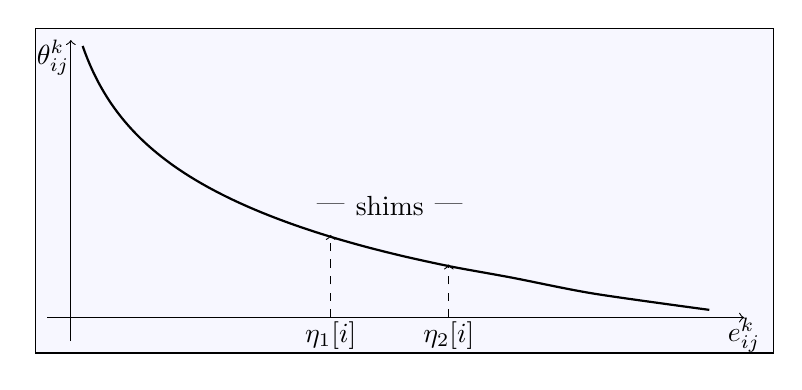
\begin{tikzpicture}[scale=0.75, samples=100]
			\filldraw[fill=blue!3!white, draw=black] (0, 0) rectangle (12.5, 5.5);
			\draw[->] (.2, .6) -- coordinate (x axis mid) (12, .6);
			\node at (5, 0.3) {$\eta_1[i]$};
			\node at (5, 2.5) {|};
			\node at (6, 2.5) {shims};
			\node at (7, 2.5) {|};
			\node at (7, 0.3) {$\eta_2[i]$};
			\node at (0.3, 5) {$\theta_{ij}^k$};
			\draw[->] (.6, .2) -- coordinate (y axis mid) (0.6, 5.3);
			\node at (12, 0.3) {$e_{ij}^k$};
			\draw[smooth, domain = 0.09:2, color=black, thick] plot (.3+1/\x,{4.2+log2(\x)});
			\draw[->, dashed] (5, 0.6)--(5, 2.0);
			\draw[->, dashed] (7, 0.6)--(7, 1.5);
		\end{tikzpicture}
		
		\captionof{figure}{$n_k$\/ edges $e_{ij}^k$\/ of $p_i$\/ sorted by $\theta_{ij}^k$\/ in non-ascending order}
		\label{fig:whip}		
	\end{minipage}
\end{table}



In this heuristic, described in Algorithm \ref{alg:shims}, pallets $p_i$\/ are considered in non-descending order of $|p_i.d|$ (line \ref{shims:pallets}). For each $p_i$, the $n_k$\/ possible edges $e_{ ij}^k$\/ are considered in non-increasing order of $\theta_{ij}^k$\/ (line \ref{shims:edges}) in three phases: the greedy phase (lines \ref{shims:phase1a}-\ref{shims:phase1b}), the composition phase of the shims (lines \ref{shims:phase2a}-\ref{shims:phase2b}) and the selection phase of the best shim (lines \ref{shims:phase3a}-\ref{shims:phase3b}).

Figure \ref{fig:whip} represents the $n_k$\/ possible edges $e_{ij}^k$\/ of $p_i$\/ sorted by $\theta_{ij}^k$. \emph{Shims}\/ starts with a greedy solution, stopping at the edge with index $\eta_1[i]$ close to the local optimum (first phase). Then, considering even the edge with the index $\eta_2[i]$, it elaborates different possible complements for this pallet (second phase) and selects the best of these complements (third phase).


\begin{algorithm}[H]
	\caption{$Shims$\/ heuristic on node $k$}  \label{alg:shims}
	\begin{algorithmic}[1]
		
		\Procedure{$SolveNode$}{$Shims,\ k,\ G$}
		
		\State Let $G(V_k, E^Q_k)$
		\State Sort $M$ by $|p_i.d|$ in non-descending order \label{shims:pallets}
		\State $E^N_k \gets \varnothing$ 
		\State Let $E[1..m][1..n_k]$, where $E[i]$ is an array with $n_k$ edges $(p_i,t^k_j)$ sorted by $\theta_{ij}^k$ in non-ascending order, $1 \leq i \leq m$ \label{shims:edges}
		\State $gap \gets 2000/n_k*m$ \label{shims:gap} 
		\For{$i \gets 1$ to $m$} 
		\State $pv[i] \gets 0$		\label{shims:phase1a}
		\State $\eta_1[i] \gets 0$
		\While{($p_i.v - pv[i] > gap*p_i.v$) {\bf and} ($\eta_1[i]<n_k$)} \label{shims1:slack}
		\State $\eta_1[i] \gets \eta_1[i] + 1$ \label{shims:eta1}
		\State $e^k_{ij} \gets E[i][\eta_1[i]]$
		\If{($e^k_{ij}$ is feasible) {\bf and} ($t^k_j.v \leq p_i.v - pv[i]$)} 
		\State $E^N_k \gets E^N_k \cup \{e^k_{ij}\}$
		\State $pv[i] \gets pv[i] + t^k_j.v$ 
		\EndIf
		\EndWhile 
		\State $slack[i] \gets p_i.v - pv[i]$
		\State $\eta_2[i] \gets \eta_1[i]$
		\Repeat
		\State $\eta_2[i] \gets \eta_2[i] + 1$  \label{shims:eta2}
		\State $e^k_{ij} \gets E[i][\eta_2[i]]$
		\State $pv[i] \gets pv[i] + t^k_j.v$
		\Until{($\eta_2[i] = n_k$) {\bf or} ($ pv[i] \geq (1 + 3*gap)*p_i.v)$)} \label{shims:phase1b}
		\State $Set \gets \varnothing$  \label{shims:phase2a}
		\State $q \gets 1$
		\State $shim[q] \gets \varnothing$
		\State $volume \gets 0$
		\For{$x \gets \eta_1[i]$ to $\eta_2[i]$}
		\State $e_{ij}^k \gets E[i][x]$
		\If {($e_{ij}^k \not\in E^N_k \cup shim[q]$) {\bf and} ($e_{ij}^k$ is feasible)}
		\If{$t_j^k.v + volume \leq slack[i]$} \label{bincapacity}
		\State $shim[q] \gets shim[q] \cup \{e_{ij}^k\}$	
		\State $volume \gets volume + t_j^k.v$	
		\Else \label{newbins}
		\State $Set \gets Set \cup shim[q] $
		\State $q \gets q+1$
		\State $shim[q] \gets \varnothing$
		\State $volume \gets 0$
		\If{$t_j^k.v \leq slack[i]$} 
		\State $shim[q] \gets shim[q] \cup \{e_{ij}^k\}$	
		\State $volume \gets volume + t_j^k.v$
		\EndIf
		\EndIf
		\EndIf
		\EndFor   \label{shims:phase2b}
		\State $sh_w \gets S$, where $S \in Set$ and $\sum_{e_{ab}^k \in S} t_b^k.w$ is maximum \label{shims:phase3a}
		\State $sh_v \gets S$, where $S \in Set$ and $\sum_{e_{ab}^k \in S} t_b^k.v$ is maximum
		\State $sh_{best} \gets S$, where $S \in \{sh_w, sh_v\}$ and $\sum_{e_{ab}^k \in x} t_b^k.s$ is maximum
		\State $E^N_k \gets E^N_k \cup sh_{best}$ \label{shims:phase3b}
		\EndFor
		\Return $G(V_k, E^N_k \cup E^Q_k)$
		\EndProcedure
	\end{algorithmic}
\end{algorithm}

In the first phase (lines \ref{shims:phase1a}-\ref{shims:phase1b}), a greedy and partial solution for $p_i$\/ is constructed by edges inclusion, until a certain slack or clearance is reached. This slack was empirically defined as $gap * p_i.v$\/ (line \ref{shims1:slack}), where $gap = 2000/n_k*m$\/ (line \ref{shims:gap}).

In the second phase (lines \ref{shims:phase2a}-\ref{shims:phase2b}), a set of shims named $Set$\/ is created, where each shim is formed by a group of edges in the range $[\eta_1[i],\eta_2[i]]$, whose total volume is limited by $slack[i]$. In this phase, the heuristic that provided the best results, both in terms of time and quality, is based on {\it Next-Fit}, which is an approximation algorithm for the {\it Bin Packing Problem}\/ \cite{JohnsonGarey1985}. Basically, shims are created by accumulating the following edges, taking $slack[i]$\/ as a limit.

In the third phase (lines \ref{shims:phase3a}-\ref{shims:phase3b}), the best shim in $Set$\/ is chosen. Initially, two shims are found: $sh_w$\/ with larger weight and $sh_v$\/ with larger volume. Among the two, the shim with the highest score will be chosen and its edges are inserted into $E^N_k$.






\section{Implementation and results}
\label{sec6}

This section is composed of two parts: the generation of test instances and the results obtained in our implementation.


\subsection{Instances generation}
\label{items}

As we are dealing with a new problem, which until now had not been modeled in the literature, we have to create our own benchmarks. For this, we based on the characteristics of real airlifts carried out by the {\it Brazilian Air Force}, as described below.

In the military airlift carried out in Brazil from 2008 to 2010, 23\% of the items weighed between $10kg$ and $20kg$, 22\% from $21kg$ to $40kg$, 24\% from $41kg$ to $80kg$, 23\% from $81kg$ to $200kg$, and 8\% between $201kg$ and $340kg$. These five groups of items are described in Table \ref{tab:weights}, where $P$\/ represents the group probability. On the other hand, the average density of these items is approximately $246 kg/m^3$.

\begin{table}[H]
		\centering
		\caption{Items weight distribution ($kg$) in Brazil}  \label{tab:weights}
		\begin{tabular}{c c c c }
			\toprule
			$Group$ & $P$ & $low$ & $high$  \\		
			\midrule
			1              & 0.23           & 10  & 20  \\
			2              & 0.22           & 21  & 40  \\
			3              & 0.24           & 41  & 80  \\		
			4              & 0.23           & 81  & 200 \\
			5              & 0.08           & 201 & 340 \\
			\bottomrule
		\end{tabular}
\end{table}


In the generation of test instances, we use three types of random selections:
\begin{itemize}
	\item $RandomReal(r_1,r_2)$: randomly selects a real number in $[r_1,r_2]$, where $r_1$ and $r_2$ are real numbers;
	\item $RandomInt(i_1,i_2)$: randomly selects a integer number in $[i_1,i_2]$, where $i_1$ and $i_2$ are integer numbers;
	\item $Roulette(set)$ biased through $\phi$: selects an element from $set$, where the probability of each element is proportional to the value of a given function $\phi$\/ defined on $set$.
\end{itemize}

$ItemsGeneration$, which generates $N$, is described in Algorithm \ref{alg:itemsgen}. The parameter $scenario$\/ defines $L$\/ and $M$\/ (line \ref{ig:LM}), and the parameter $volume$\/ sets a limit on the total volume of items at each node (line \ref{ig:extended}). To avoid simply loading all items, we use $volume > 1$.

\begin{algorithm}[H]
	\caption{Procedure to generate items}  \label{alg:itemsgen}
	\begin{algorithmic}[1]
		
		\Procedure{$ItemsGeneration$}{$scenario,\ volume$}
		
		\State Let $L$ and $M$ be according to $scenario$ \label{ig:LM}
		\State $limit \gets volume \times \sum_{i=1}^{m} p_i.v$ \label{ig:extended}
		\For{$k \gets 0$ to $K$}
			\State $N_k \gets \varnothing$
			\State $j \gets 0$
			\State $vol \gets 0$	\label{ig:totals}	
			\While{$vol < limit$}
				\State $j \gets j+1$
				\Repeat
					\State $t_j^k.to \gets RandomInt(0, K)$ \label{ig:dest}
				\Until{$t_j^k.to \neq k$}
				\State $x = Roulette(item)$ biased through $P$ \label{ig:weight1} \Comment{From Table \ref{tab:weights}}	
				\State $t_j^k.w \gets RandomReal(low(x), high(x))$        \label{ig:weight2}		
				\State $t_j^k.s \gets \round{100 \times (1 - \log_{10}(RandomInt(1, 9)))} $ \label{ig:score}
				\State $t_j^k.v \gets t_j^k.w / RandomReal(148, 344)$ \label{ig:volume}
				\State $vol \gets vol + t_j^k.v$ 
				\State $N_k \gets N_k \cup \{t_j^k\}$ 
			\EndWhile
			\State $n_k \gets j$
		\EndFor
		\State $N \gets \bigcup_{0 \leq k \leq K} N_k$ 
		\Return $N$
		\EndProcedure
	\end{algorithmic}
\end{algorithm}

For each generated $t^k_j$\/ item, its destination is uniformly random selected (line \ref{ig:dest}), its weight has a distribution according to Table \ref{tab:weights} (lines \ref{ig:weight1}-\ref{ig:weight2}), its score varies $100$\/ (highest) and $5$\/ (lowest) according to a logarithmic scale (line \ref{ig:score}, and its volume is randomly defined from the density, where we allow a variation of 40\% more or less than the average density of $246 kg/m^3$\/ (line \ref{ig:volume}).


\subsection{Results obtained}

In the tests performed, we used a 64-bit, 16GB, 3.6GHz, eight-core processor with {\it Linux Ubuntu 22.04.1 LTS 64-bit} as the operational system and {\it Python 3.10.4}\/ as the programming language. We also used the well-known solver {\it Gurobi}\/ (www.gurobi.com), version 9.5.2.

We ran Algorithm \ref{alg:main} in the 6 scenarios described in Table \ref{tab:scenarios}, considering 6 methods for node-by-node resolution: Gurobi (see \ref{solver}), ACO, NMO, TS, GRASP, and Shims (Algorithm \ref{alg:shims}). In generating the items in each node, we consider 3 values for the parameter $volume$. The results obtained for the function $f$, with the corresponding runtime in seconds, are shown in Tables \ref{tab:20} ($volume = 1.2$), \ref{tab:50} ($volume = 1.5$) and \ref{tab:100} ($volume = 2.0$). For each $method$, $scenario$\/ and $volume$, 7 different instances were generated. Therefore, 126 tests (6 scenarios $\times$\/ 3 volumes $\times$\/ 7 instances) were performed for each method. 

The average values were presented for $f$\/ and, for the runtime, the worst result obtained. To facilitate the comparison between the methods, we added a last column in these tables, where two values are indicated:
\begin{itemize}
\item {\bf Normalized}: value between 0 and 1, which corresponds to the ratio between the sum of $f$\/ values obtained by the method in all scenarios and the sum of the best values obtained among all methods in all scenarios. The higher the value of {\bf Normalized}, the closer the method approached the best solutions found.
\item {\bf Speed-up}: ratio of the sums of the worst runtimes of all scenarios and the sum of the method runtimes in all scenarios. The method with the highest {\bf Speed-up}\/ is the fastest.
\end{itemize}

In each $scenario$, we indicate in bold the best value of $f$\/ found. In each table, we also indicate in bold the best {\bf Normalized}\/ and {\bf Speed-up}\/ values.


\begin{table}[H]
	\centering
	\caption{Methods and scenarios with $volume =1.2$}  \label{tab:20}
	\footnotesize
	\begin{tabular}{c|c|cccccc|c}
		\toprule
		{$method$}                        & {\bf Results}    & {\bf 1}     &  {\bf 2}    & {\bf 3}      & {\bf 4}      & {\bf 5}      & {\bf 6}     & \specialcell{{\bf Normalized}\\{\bf Speed-up}}  
		\\
		\toprule
		\multirow{2}{*}{\textbf{Gurobi}}  & $f$      & {\bf 10.76} & 6.10  & {\bf 10.02}& {\bf 10.82} & {\bf 12.13} & {\bf 12.10} & {\bf 0.998} \\
		&{\bf runtime (s)} & 6         & 14     & 51        & 243       & 1,417     & 9,720     &  1.000 \\ 
		\midrule[.1pt]
		\multirow{2}{*}{\textbf{TS}}      & $f$     & 8.88       & 6.56     & 8.49       & 9.19       & 11.25      & 11.48      &  0.900 \\
		&{\bf runtime (s)}& 4         & 4       & 17        & 86        & 516       & 3,600     &  2.709 \\ 
		\midrule[.1pt]		
		\multirow{2}{*}{\textbf{GRASP}}   & $f$   & 9.30       & 6.76     & 8.85       & 9.65       & 11.75      & 11.54      &  0.932 \\ 
		&{\bf runtime (s)}& $<1$         & 4       & 17        & 80        & 472       & 3,265     &  2.984 \\ 
		\midrule[.1pt]
		\multirow{2}{*}{\textbf{ACO}}     & $f$      & 9.43       & {\bf 6.77}& 8.85      & 9.65       & 11.75      & 11.54      &  0.934 \\ 
		&{\bf runtime (s)}& 3         & 4        & 17       & 86        & 513       & 3,596     &  2.714 \\ 
		\midrule[.1pt]	
		\multirow{2}{*}{\textbf{NMO}}     & $f$     & 9.15       & 6.74      & 8.80      & 9.61       & 11.76      & 11.50      &  0.928 \\
		&{\bf runtime (s)}& $< 1$         & 4        & 17       & 86        & 508       & 3,480     &  2.796 \\ 
		\midrule[.1pt]	
		\multirow{2}{*}{\textbf{Shims}}   & $f$     & 10.18       & {\bf 6.77} & 8.92     & 9.60       & 11.78      & 11.61      &  0.948       \\ 
		&{\bf runtime (s)}& $< 1$         & 2         & 8       & 31        & 166       & 1,087     &  {\bf 8.856} \\ 
		\bottomrule
	\end{tabular}
	\normalsize
\end{table}



\begin{table}[H]
	\centering
	\caption{Methods and scenarios with $volume =1.5$}  \label{tab:50}
	\footnotesize
	\begin{tabular}{c|c|cccccc|c}
		\toprule
		{$method$}                        & {\bf Results}   & {\bf 1}     &  {\bf 2}    & {\bf 3}      & {\bf 4}      & {\bf 5}      & {\bf 6}     & \specialcell{{\bf Normalized}\\{\bf Speed-up}} \\
		\toprule
		\multirow{2}{*}{\textbf{Gurobi}}  & $f$     & {\bf 15.90}& 4.756       & 8.84        & 11.94       & 16.21       &{\bf 16.47} & 0.881  \\	 
		&{\bf runtime (s)}& 6         & 18        & 68         & 326        & 1,906      & 12,960    & 1.000  \\	 
		\midrule[.1pt]
		\multirow{2}{*}{\textbf{TS}}      & $f$     & 12.40      & 8.97       & 11.44       & 12.92       & 15.20       & 15.39      &  0.907 \\		
		&{\bf runtime (s)}& 4         & 4         & 18         & 88         & 525        & 3,660     &  3.555  \\		
		\midrule[.1pt]		
		\multirow{2}{*}{\textbf{GRASP}}   & $f$    & 13.12      & 9.36       & 12.34       & 13.63       & 16.18       & 15.44      &  0.951 \\ 
		&{\bf runtime (s)}& $< 1$         & 4         & 17         & 86         & 515        & 3,564     &  3.651  \\
		\midrule[.1pt]	
		\multirow{2}{*}{\textbf{ACO}}     & $f$      & 13.17      & 9.36       & 12.34       & 13.63       & 16.18       & 15.44      &  0.952 \\
		&{\bf runtime (s)}& 4         & 5         & 19         & 90         & 539        & 3,720     &  3.492  \\	
		\midrule[.1pt]	
		\multirow{2}{*}{\textbf{NMO}}     & $f$     & 12.94      & 9.36       & 12.33       & 13.60       & 16.16       & 15.43      &  0.948 \\ 
		&{\bf runtime (s)}& 2         & 5         & 19         & 91         & 544        & 3,780     & 3.442  \\
		\midrule[.1pt]	
		\multirow{2}{*}{\textbf{Shims}}   & $f$     & 14.15      & {\bf 9.39} & {\bf 12.42} & {\bf 13.72} & {\bf 16.28} & 15.49      &  {\bf 0.968} \\	
		&{\bf runtime (s)}& $< 1$         & 3         & 11         & 48         & 265        & 1,720     &  {\bf 7.470}  \\
		\bottomrule
	\end{tabular}
	\normalsize
\end{table}


\begin{table}[H]
	\centering
	\caption{Methods and scenarios with $volume = 2.0$}  \label{tab:100}
	\footnotesize
	\begin{tabular}{c|c|cccccc|c}
		\toprule
		{$method$}                        & {\bf Results}    & {\bf 1}     &  {\bf 2}   & {\bf 3}    & {\bf 4}    & {\bf 5}     & {\bf 6}     & \specialcell{{\bf Normalized}\\{\bf Speed-up}} \\
		\toprule
		\multirow{2}{*}{\textbf{Gurobi}}  & $f$     &{\bf 22.45} & 4.92      & 6.58      & 6.34       & 7.24       & 8.15      &  0.457 \\ 
		&{\bf runtime (s)}& 8         & 29       & 106      & 493      & 2,833     & 19,380      &  1.000  \\ 
		\midrule[.1pt]
		\multirow{2}{*}{\textbf{TS}}      & $f$    & 18.87      & 13.72     & 17.53     & 19.28     & 21.78      & 22.35      &  0.929 \\		
		&{\bf runtime (s)}& 4         & 5        & 19       & 93       & 556       & 3,900     &  4.992  \\	
		\midrule[.1pt]		
		\multirow{2}{*}{\textbf{GRASP}}   & $f$    & 19.36      & 13.99     & 19.39     & 19.86     & 23.50      & 22.57      &  0.973 \\
		&{\bf runtime (s)}& 2         & 6        & 21       & 97       & 571       & 3,960     &  4.906  \\	
		\midrule[.1pt]
		\multirow{2}{*}{\textbf{ACO}}     & $f$    & 19.36      & 13.99     & 19.39     & 19.86     & 23.50      & 22.57      &  0.973 \\
		&{\bf runtime (s)}& 4         & 6        & 23       & 105      & 597       & 4,080     &  4.745  \\	
		\midrule[.1pt]	
		\multirow{2}{*}{\textbf{NMO}}     & $f$    & 18.85      & 13.99     & 19.39     & 19.85     & 23.50      & 22.56      & 0.969 \\	
		&{\bf runtime (s)}& 4         & 9        & 27       & 120      & 681       & 4,620     & 4.184  \\	
		\midrule[.1pt]	
		\multirow{2}{*}{\textbf{Shims}}   & $f$     & 20.46      &{\bf 14.00} & {\bf 19.44} & {\bf 19.94} & {\bf 23.55} & {\bf 22.58} & {\bf 0.984} \\	
		&{\bf runtime (s)}& $< 1$         & 7        & 20       & 84       & 450       & 2,918     & {\bf 6.570}  \\
		\bottomrule
	\end{tabular}
	\normalsize
\end{table}

In Tables \ref{tab:20}, \ref{tab:50} and \ref{tab:100}, $Gurobi$\/ was the slowest method and $Shims$\/ was the fastest. This was expected, as $Gurobi$\/ is a MIP solver, which seeks an optimal solution within the established constraints, usually reaching its time limit on each node, while {\it Shims} is a fast heuristic. This way, $Gurobi$\/ even demands prohibitive times (more than 5 hours in scenario 6 of Table \ref{tab:100}), while the maximum time required by $Shims$\/ did not reach one hour.

Considering the {\bf Normalized}\/ values, in Table \ref{tab:20} $Gurobi$\/ was the best ($0.998$), followed closely by $Shims$\/ ($0.948$). In Tables \ref{tab:50} and \ref{tab:100}, $Shims$ was the best ($0.968$\/ and $0.984$). As expected, the performance of $Gurobi$\/ drops sharply as the volume of shipments at the nodes increases: $0.881$\/ in Table \ref{tab:50} and $0.457$\/ in Table \ref{tab:100}.

It is worth noting that the other heuristics always obtained {\bf Normalized}\/ values greater than or equal to $0.9$, and were always faster than $Gurobi$.



\section{Conclusions}
\label{sec7}

In this work, we modeled and solved a real air transport problem, named {\it Air Cargo Load Planning with Routing, Pickup and Delivery Problem}\/ (ACLP+RPDP). For the first time in the literature, an NP-hard problem that involves {\it simultaneously}\/ pallet assembly, load balancing and route planning is addressed, where the cost-effectiveness of transport is maximized. We adopted some simplifications that are not critical, but that allowed the unprecedented resolution of this problem considering more than two nodes.

We consider that, in practical cases, the number $K$\/ of nodes, excluding the base, is small ($K \leq 6$), each of them with hundreds of items to be shipped. Thus, considering real aircraft models, we developed some node-by-node heuristics, which allow us to enumerate all $K!$\/ tours and choose the best. The complete process can be executed quickly on a simple handheld computer, offering good results and reducing stress for the transport planners. As validation, we performed tests in several scenarios with real data from {\it Brazilian Air Force}.

In less than one hour, this development can establish a near optimal distribution of load on pallets to be put in the cargo bay, enforcing the loaded aircraft balance, maximizing the total score and minimizing fuel consumption for the airlift. The output, which includes the tour plan and the pallet building and arrangement plan, is an essential part of airlift: it improves flight safety, makes ground operations more efficient, and makes sure that each item gets to its right destination.

Our main contribution was the mathematical modeling of this complex problem, which involves four NP-hard subproblems, and a complete process that offers a fast and good-quality solution. As future work, we intend to include dimensions in the items, and consider the use of multiple aircraft or load sequencing in an aircraft with two doors.

The simple heuristic $Shims$\/ presented the best node-by-node results in a restricted time interval. Without it, it would not be possible to test all routes: after all, the greater the number of nodes, the shorter the runtime limit for node-by-node resolution. We also show that, as the shipment volume increases, the exact node-by-node resolution becomes unfeasible, indicating the importance of a fast and good-quality heuristic.

Finally, by focusing on node-by-node resolution, the result of this work is not exclusive to aircraft and airports: it can be adapted, for example, to ships and ports, or vehicles and warehouses, or freight cars and railways. In these cases, it would be necessary to make some changes in the modeling: for example, modify the load balancing constraints, and consider the available space in vehicles or freight cars instead of pallets.

\section*{Acknowledgments}

This research was partially supported by \textit{S�o Paulo Research Foundation} (FAPESP, grant 2016/01860-1).

\begin{thebibliography}{00}

\bibitem{LarsenMikkelsen1979} O. Larsen and G. Mikkelsen, An interactive system for the loading of cargo aircraft, {\it European Journal of Operational Research}, Vol. 4 (6), pp. 367-373, 1980.

\bibitem{Brosh1981} I. Brosh, Optimal cargo allocation on board a plane: a sequential linear programming approach, {\it European Journal of Operational Research}, Vol. 8 (1), pp. 40-46, 1981.

\bibitem{JohnsonGarey1985} D.S. Johnson and M.R. Garey, A 71/60 theorem for bin packing, {\it Journal of Complexity}, Vol. 1 (1), pp. 65-106, 1985.

\bibitem{Glover1986} F. Glover, Future paths for integer programming and links to artificial intelligence, {\it Computers and Operations Research}, Vol. 13, pp. 533-549, 1986.

\bibitem{FeoResende1989} T.A. Feo and M.G.C. Resende, A probabilistic heuristic for a computationally difficult set covering problem, {\it Operations Research Letters}, Vol. 8 (2), pp. 67-71, 1989.

\bibitem{Kevin1992} K.Y.K. Ng, A multicriteria optimization approach to aircraft loading, {\it Operations Research}, Vol. 40 (6), pp. 1200-1205, 1992.

\bibitem{Dorigo1992} M. Dorigo, {\it Optimization, Learning and Natural Algorithms}, PhD Thesis, Politecnico di Milano, 1992.

\bibitem{CharonHudry1993} I. Charon and O. Hudry, The noising method: a new method for combinatorial optimization, {\it Operations Research Letters}, Vol. 14 (3), pp. 133-137, 1993.

\bibitem{DorigoManiezzoColorni1996} M. Dorigo, V. Maniezzo and A. Colorni, The ant system: optimization by a colony of cooperating agents, {\it IEEE Transactions on Systems, Man, and Cybernetics}, Vol. 26 (1), pp. 29-41, 1996.

\bibitem{NiarFreville1997} S. Niar and A. Freville, A parallel tabu search algorithm for the 0-1 multidimensional knapsack problem, Proceedings of {\it 11th International Parallel Processing Symposium}, 1997.

\bibitem{Heidelberg1998} K.R. Heidelberg, G.S. Parnell and J.E. Ames, Automated air load planning, {\it Naval Research Logistics}, Vol. 45 (8), pp. 751-768, 1998.

\bibitem{CharonHudry2001} I. Charon and O. Hudry, The noising methods: a generalization of some metaheuristics, {\it European Journal of Operational Research}, Vol. 135 (1), pp. 86-101, 2001.

\bibitem{MongeauBes2003} M. Mongeau and C. Bes, Optimization of aircraft container loading, {\it IEEE Transaction on Aerospace and Electronic Systems}, Vol. 39 (1), pp. 140-150, 2003.

\bibitem{fok2004optimizing} K. Fok and A. Chun, Optimizing air cargo load planning and analysis, Proceedings of {\it The International Conference on Computing, Communications and Control Technologies}, 2004.

\bibitem{Fidanova2006} S. Fidanova, Ant colony optimization and multiple knapsack problem and model bias, {\it Numerical Analysis and Its Applications}, Springer Berlin Heidelberg, pp. 280-287, 2005.
	
\bibitem{Chan2006} F.T.S. Chan, R. Bhagwat, N. Kumar. M.K. Tiwari and P. Lam, Development of a decision support system for air-cargo pallets loading problem: a case study, {\it Expert Systems with Applications}, Vol. 31 (3), pp. 472-485, 2006.

\bibitem{KaluznyBohdanL2009Oalb} B.L. Kaluzny and R.H.A.D. Shaw, Optimal aircraft load balancing, {\it International Transactions in Operational Research}, Vol. 16 (6), pp. 767-787, 2009.

\bibitem{MesquitaCunha2011} A.C.P. Mesquita and C.B. Cunha, An integrated heuristic based on the Scatter Search metaheuristic for vehicle routing problems with simultaneous delivery and pickup in the context of the Brazilian Air Force, {\it Transportes}, Vol. 19, pp. 33-42, 2011.

\bibitem{Verstichel2011} J. Verstichel, W. Vancroonenburg, W. Souffriau and G.V. Berghe, A mixed integer programming approach to the aircraft weight and balance problem, {\it Procedia Social and Behavioral Sciences}, Vol. 20, pp. 1051-1059, 2011.

\bibitem{Limbourg2012} S. Limbourg, M. Schyns and G. Laporte, Automatic aircraft cargo load planning, {\it Journal of the Operational Research Society}, Vol. 63 (9), pp. 1271-1283, 2012.

\bibitem{RoesenerHall2014} A.G. Roesener and S. Hall, A nonlinear integer programming formulation for the airlift loading problem with insufficient aircraft, {\it Journal of Nonlinear Analysis and Optimization: Theory and Applications}, Vol. 5 (1), pp. 125-141, 2014.

\bibitem{Vancroonenburg2014} W. Vancroonenburg, J. Verstichel, K. Tavernier and G.V. Berghe, Automatic air cargo selection and weight balancing: a mixed integer programming approach, {\it Transportation Research Part E: Logistics and Transportation Review}, Vol. 65, pp. 70-83, 2014.

\bibitem{LurkinSchyns2015} V. Lurkin and M. Schyns, The airline container loading problem with pickup and delivery, {\it European Journal of Operational Research}, Vol. 244 (3), pp. 955-965, 2015.

\bibitem{RoesenerBarnes2016} A.G. Roesener and J.W. Barnes, An advanced tabu search approach to the dynamic airlift loading problem, {\it Logistics Research}, Vol. 9 (1), pp. 1-18, 2016.

\bibitem{PaquaySchynsLimbourg2016} C. Paquay, M. Schyns and S. Limbourg, A mixed integer programming formulation for the three-dimensional bin packing problem deriving from an air cargo application, {\it International Transactions in Operational Research}, Vol. 23 (1-2), pp. 187-213, 2016.

\bibitem{PaquayLimbourgSchynsOliveira2018} C. Paquay, S. Limbourg, M. Schyns and J.F. Oliveira, MIP-based constructive heuristics for the three-dimensional bin packing problem with transportation constraints, {\it International Journal of Production Research},
Vol. 56 (4), pp. 1581-1592, 2018.

\bibitem{Laabadi2018} S. Laabadi, M. Naimi, H. El Amri and B. Achchab, The 0/1 multidimensional knapsack problem and its variants: a survey of practical models and heuristic approaches, {\it American Journal of Operations Research}, Vol. 8, pp. 395-439, 2018.

\bibitem{YangLiuGao2018} Y. Chenguang, L. Hu and G. Yuan, Load planning of transport aircraft based on hybrid genetic algorithm, {\it MATEC Web of Conferences}, Vol. 179, pp. 1-6, 2018.
	
\bibitem{Alonso2019} M.T. Alonso, R. Alvarez-Valdes and F. Parreno, A GRASP algorithm for multi-container loading problems with practical constraints, {\it A Quarterly Journal of Operations Research}, Vol. 18, pp. 49-72, 2019.

\bibitem{BrandtStefan2019} F. Brandt and S. Nickel, The air cargo load planning problem - a consolidated problem definition and literature review on related problems, {\it European Journal of Operational Research}, Vol. 275 (2), pp. 399-410, 2019.

\bibitem{wong2020} E.Y.C. Wong and K.K.T. Ling, A mixed integer programming approach to air cargo load planning with multiple aircraft configurations and dangerous goods, Proceedings of {\it 7th International Conference on Frontiers of Industrial Engineering}, 2020.

\bibitem{Zhan2020} S. Zhan, L. Wang, Z. Zhang and Y. Zhong, Noising methods with hybrid greedy repair operator for 0-1 knapsack problem, {\it Memetic Computing}, Vol. 12, pp. 37-50, 2020.

\bibitem{eugene2021} E.Y.C. Wong, D.Y. Mo and S. So, Closed-loop digital twin system for air cargo load planning operations, {\it International Journal of Computer Integrated Manufacturing}, Vol. 34 (7-8), pp. 801-813, 2021.

\bibitem{zhao2021} X. Zhao, Y. Yuan, Y. Dong and R. Zhao, Optimization approach to the aircraft weight and balance problem with the centre of gravity envelope constraints, {\it IET Intelligent Transport Systems}, Vol. 15 (10), pp. 1269-1286, 2021.
	
\end{thebibliography}


\end{document}
